\chapter{Manual de usuario}

\section{Landing page e inicio de sesión}

Al acceder a la dirección web de la aplicación, aparecerá la pantalla principal.

\begin{figure}[H]
    \centering
    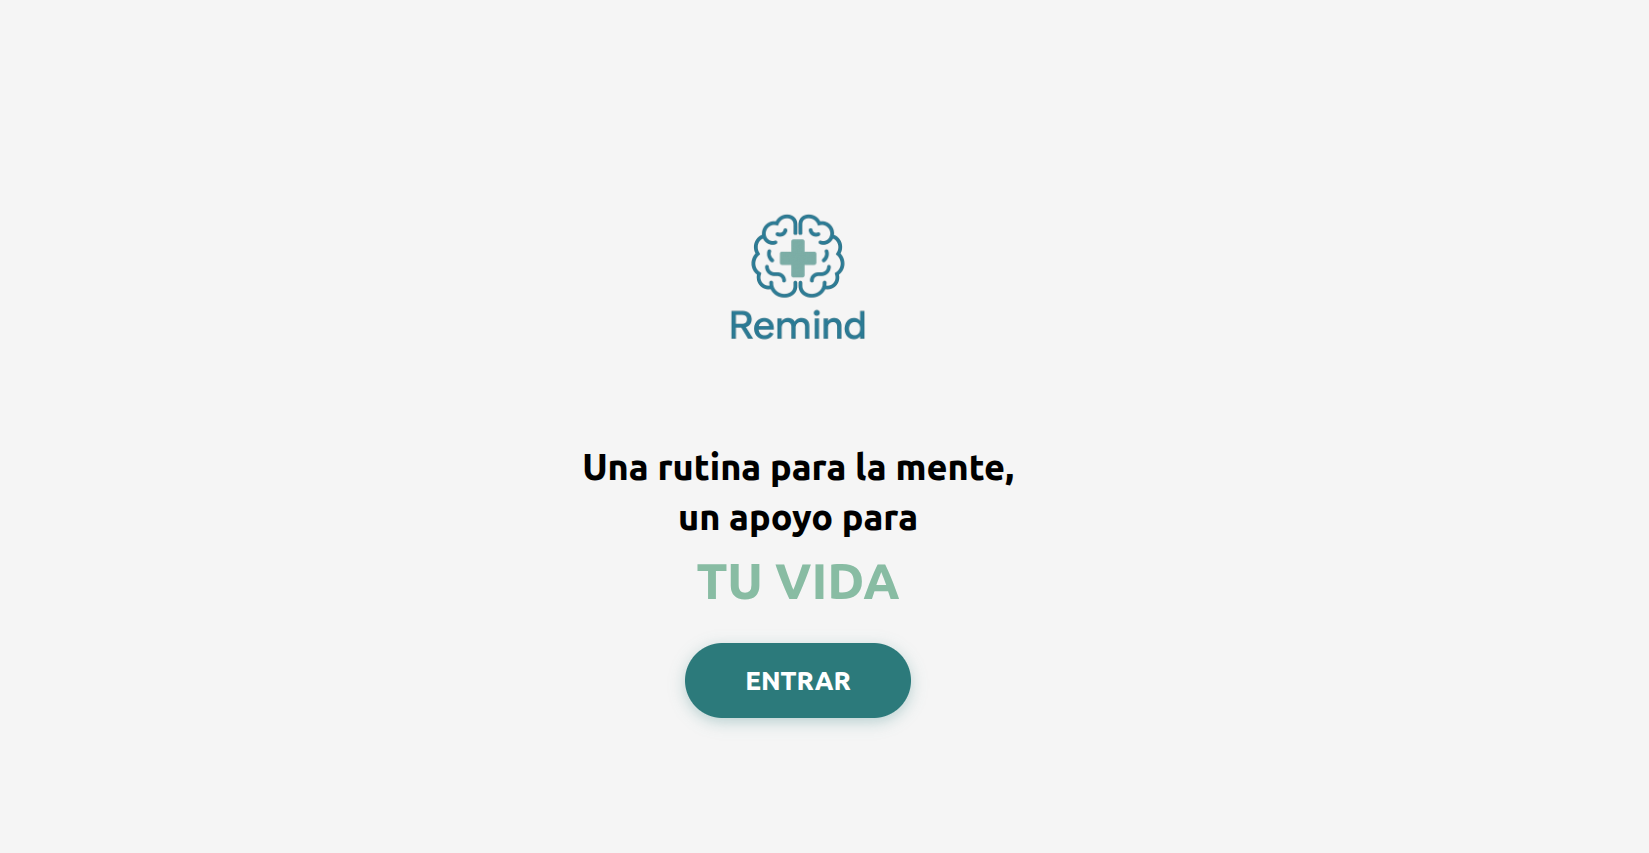
\includegraphics[width=\textwidth]{imagenes/manual/landing.png}
    \caption{Pantalla principal de la aplicación}
\end{figure}

Para entrar en la aplicación, pulse el botón \textbf{Iniciar sesión}. Se abrirá un formulario donde deberá introducir su \textbf{nombre de usuario} y su \textbf{contraseña}. Una vez escritos, pulse el botón \textbf{Iniciar sesión}.

\begin{figure}[H]
    \centering
    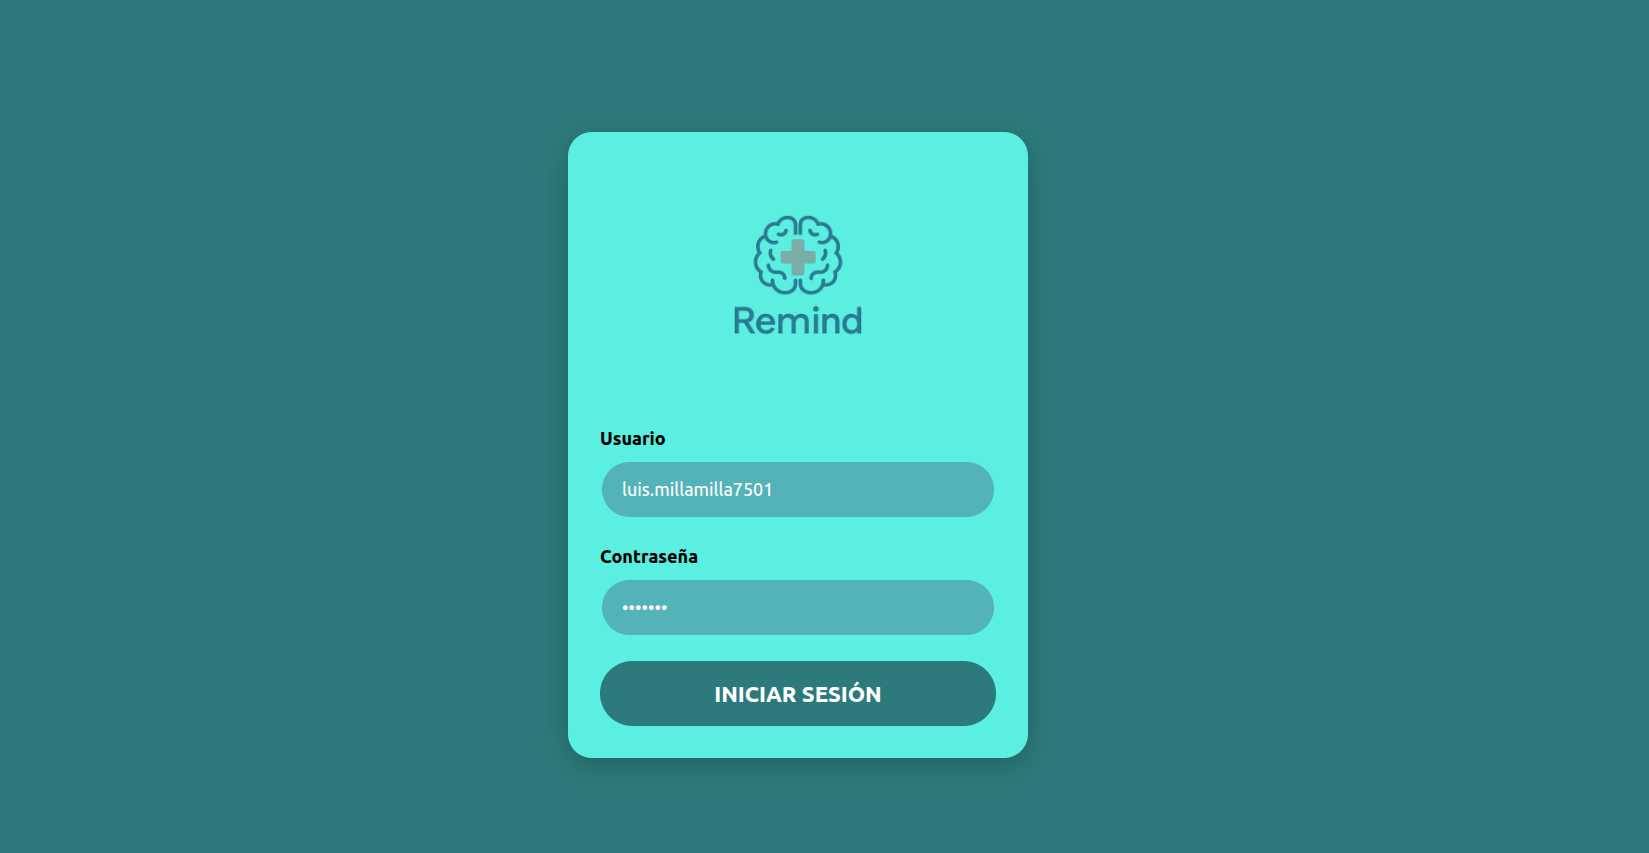
\includegraphics[width=\textwidth]{imagenes/manual/login.png}
    \caption{Pantalla de inicio de sesión}
\end{figure}

\begin{itemize}
    \item Si el usuario es \textbf{administrador}, accederá al panel de gestión de terapeutas.
    \item Si el usuario es \textbf{terapeuta}, accederá al panel de gestión de pacientes y juegos.
    \item Si el usuario es \textbf{paciente}, accederá a su agenda personal de juegos.
\end{itemize}

\begin{center}
    \fbox{\parbox{0.9\textwidth}{\textbf{Consejo:} Si tiene problemas para recordar su contraseña, consulte con su terapeuta o administrador para que le genere una nueva.}}
\end{center}

\section{Navegación general y cierre de sesión}

Todos los usuarios, independientemente de su rol, utilizan el mismo sistema de navegación. En la esquina superior izquierda de la pantalla hay un icono con tres líneas horizontales (conocido como \textbf{menú hamburguesa}). Al pulsarlo, se despliega un panel lateral con las opciones disponibles para cada rol.

\begin{figure}[H]
    \centering
    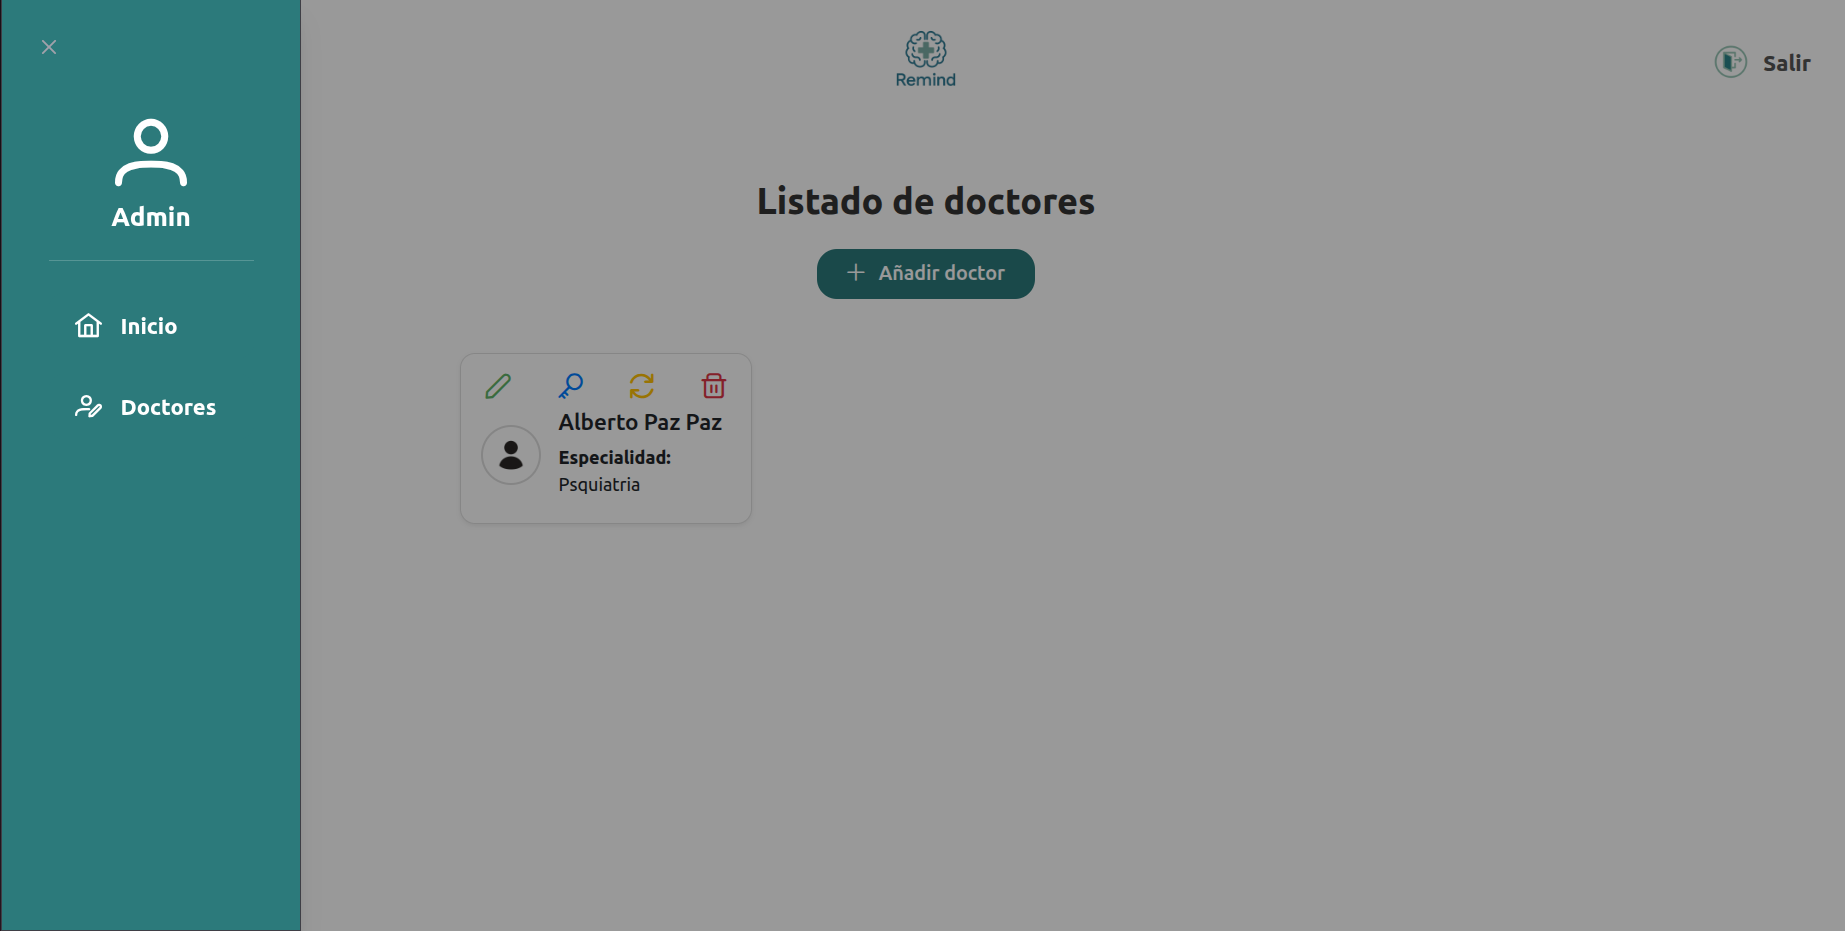
\includegraphics[width=\textwidth]{imagenes/manual/menu_admin.png}
    \caption{Ejemplo de menú de navegación desplegado}
\end{figure}

Para cerrar el menú, pulse el icono de la flecha o pulse fuera del panel. Para \textbf{cerrar la sesión}, busque la opción de salir al final del menú o pulse el botón de cierre de sesión si está visible en la pantalla principal.

\begin{center}
    \fbox{\parbox{0.9\textwidth}{\textbf{Importante:} Si está usando un dispositivo compartido (por ejemplo, en una residencia o centro de día), asegúrese de cerrar la sesión al terminar para proteger los datos del paciente.}}
\end{center}

\section{Administrador}

El administrador se encarga de gestionar los terapeutas que usarán la aplicación. Al iniciar sesión, verá su pantalla principal con un acceso directo a la gestión de doctores.

\begin{figure}[H]
    \centering
    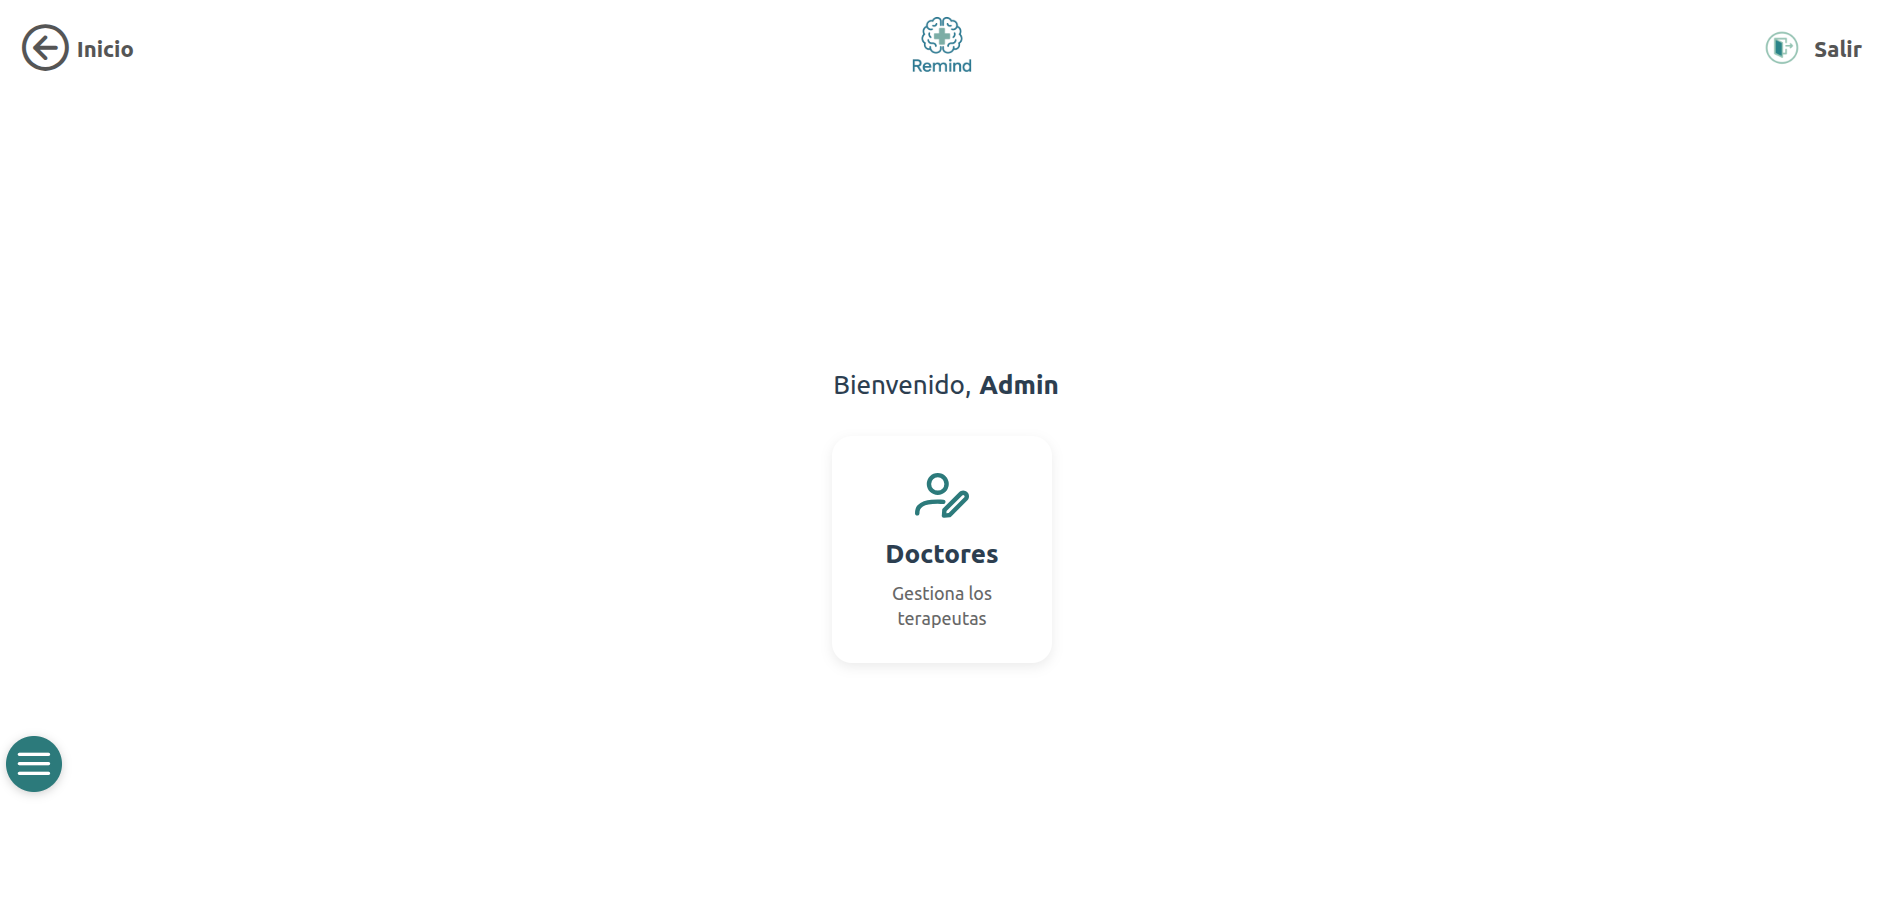
\includegraphics[width=\textwidth]{imagenes/manual/home_admin.png}
    \caption{Pantalla principal del administrador}
\end{figure}

Para navegar, pulse el icono del menú deslizable en la esquina superior izquierda. Este menú muestra las opciones disponibles según su rol.

\begin{figure}[H]
    \centering
    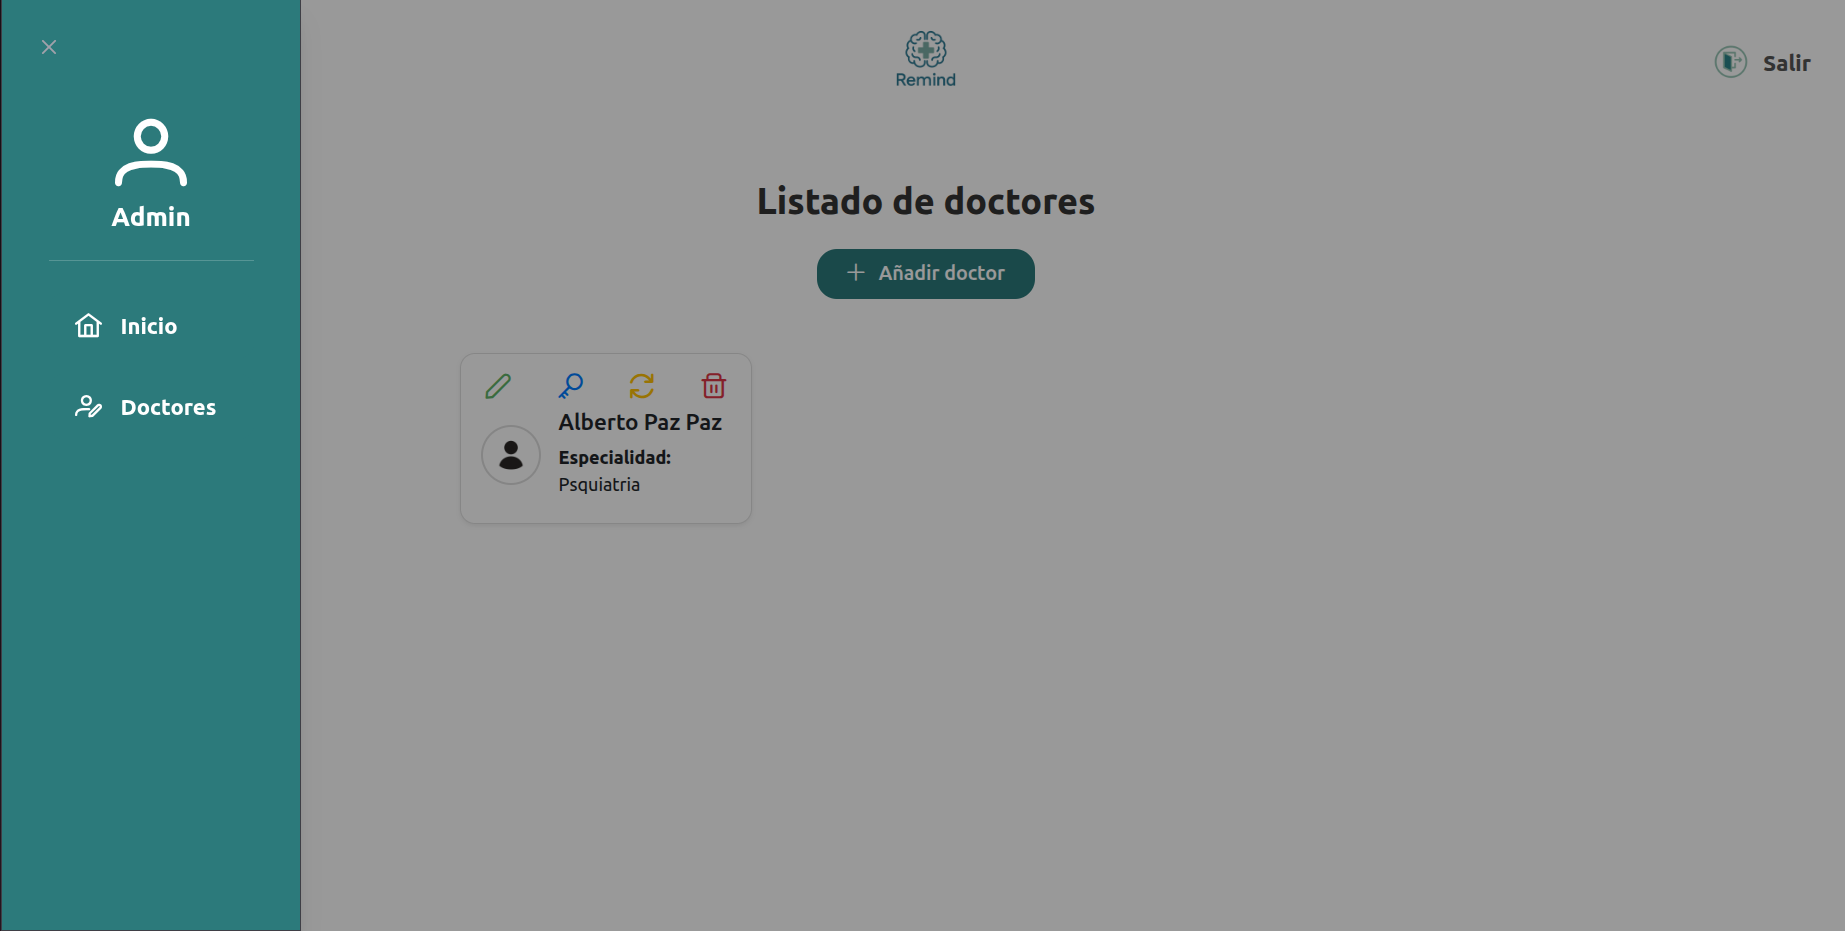
\includegraphics[width=\textwidth]{imagenes/manual/menu_admin.png}
    \caption{Menú de navegación del administrador}
\end{figure}

\subsection{Listado de terapeutas}

Al entrar en la sección de doctores, verá un listado con todos los terapeutas registrados. Desde aquí podrá añadir, editar, consultar credenciales, restablecer contraseñas y eliminar terapeutas.

\begin{figure}[H]
    \centering
    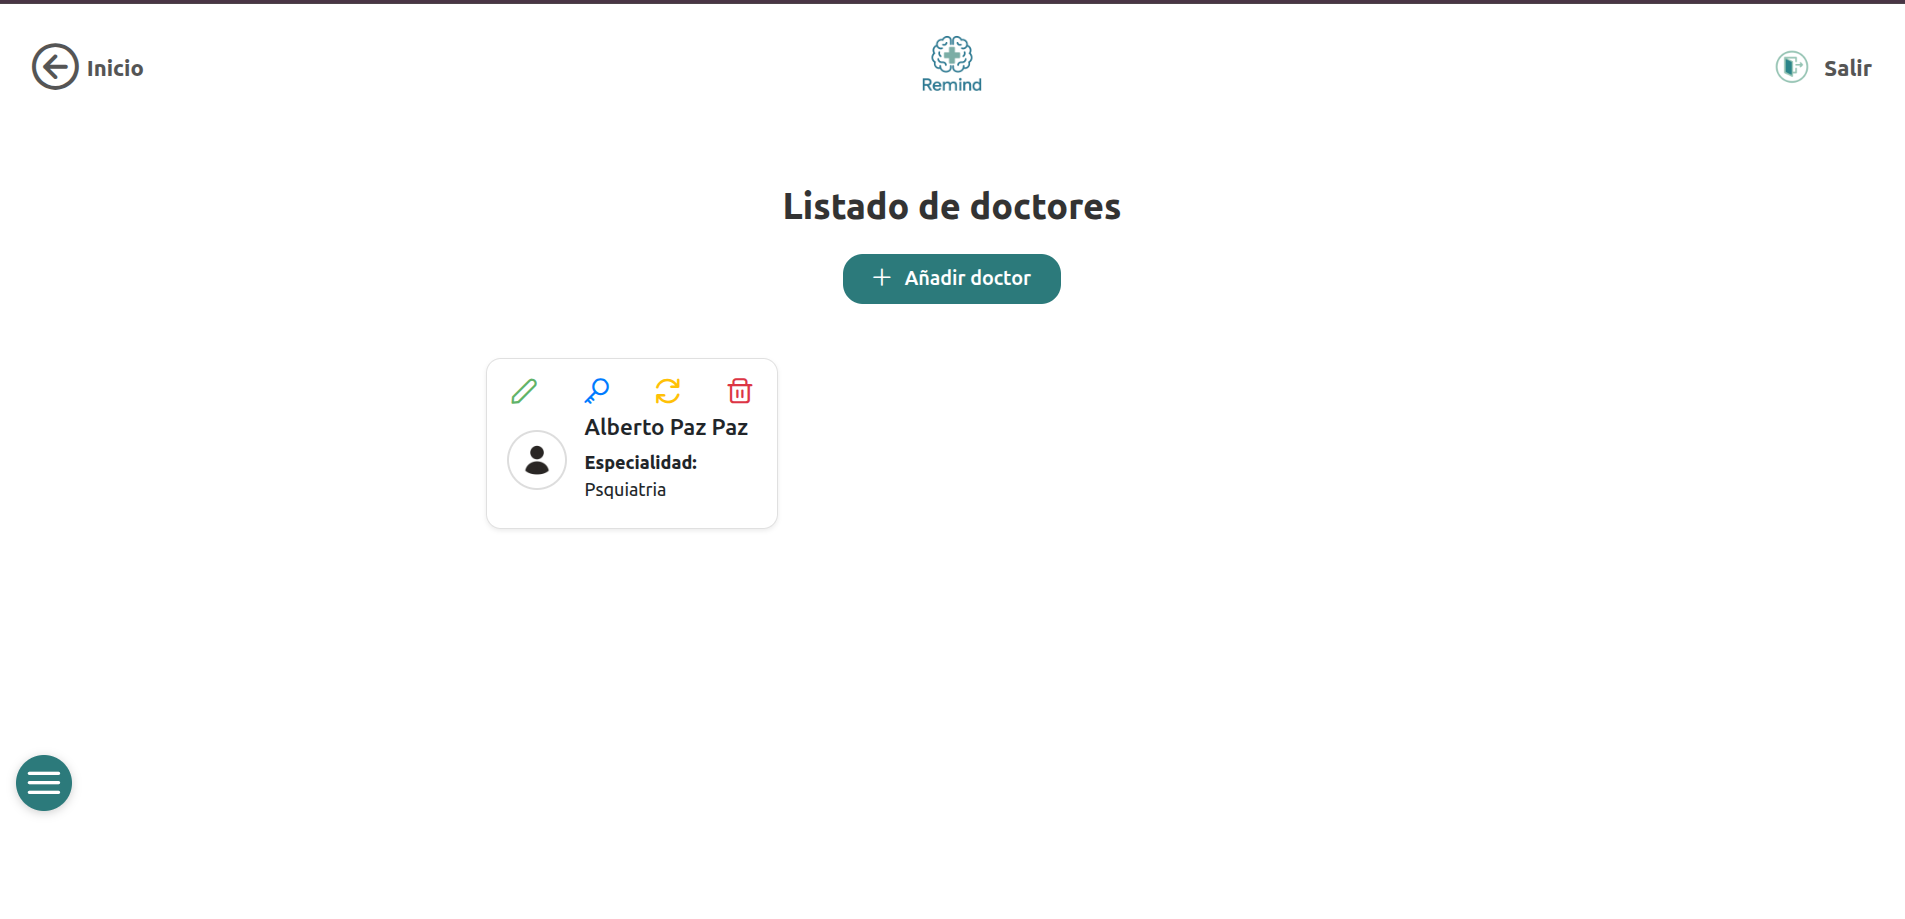
\includegraphics[width=\textwidth]{imagenes/manual/admin_doctor.png}
    \caption{Listado de terapeutas}
\end{figure}

\subsection{Crear un terapeuta}

Para dar de alta a un nuevo terapeuta, pulse el botón \textbf{Añadir doctor}. Se abrirá un formulario con los siguientes campos:

\begin{itemize}
    \item \textbf{Nombre} y \textbf{Apellidos}.
    \item \textbf{Correo electrónico}.
    \item \textbf{Teléfono de contacto}.
    \item \textbf{Especialidad} (campo opcional para indicar su área, por ejemplo: neuropsicología, terapia ocupacional, logopedia, etc.).
\end{itemize}

\begin{figure}[H]
    \centering
    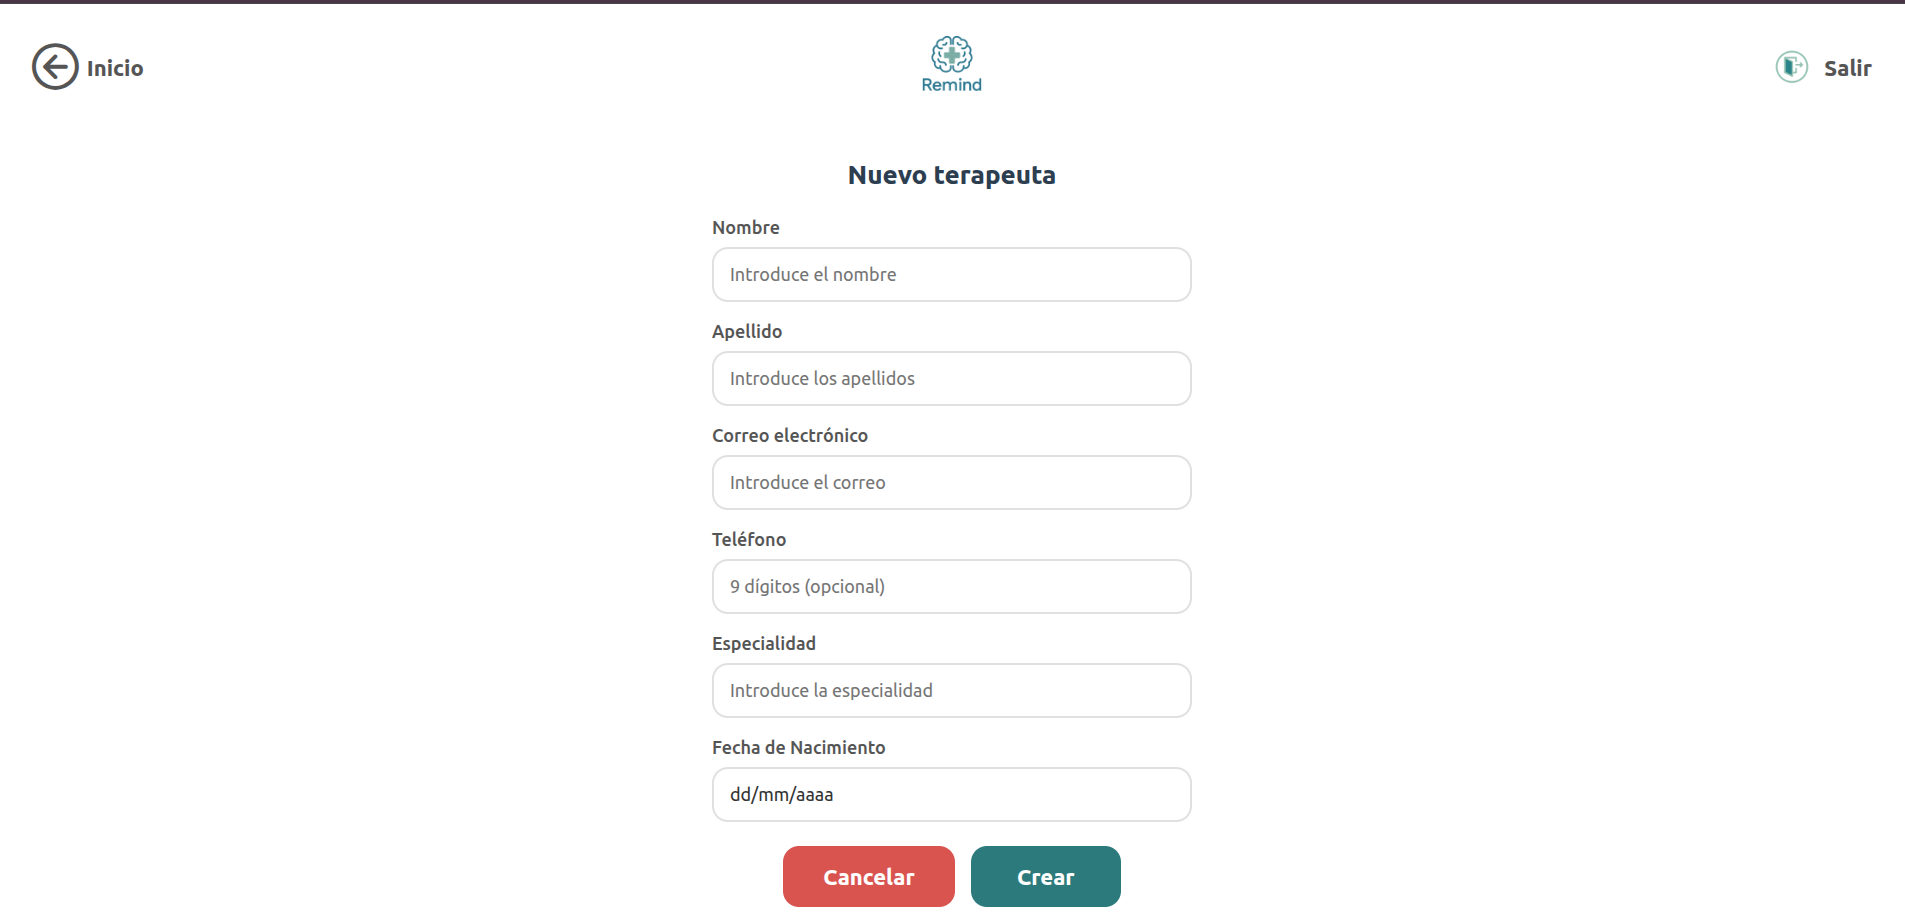
\includegraphics[width=\textwidth]{imagenes/manual/form_terapeuta.png}
    \caption{Formulario de creación de terapeuta}
\end{figure}

Rellene los datos y pulse \textbf{Guardar}. La aplicación generará automáticamente un nombre de usuario y una contraseña, y los mostrará en pantalla para que pueda comunicárselos al terapeuta.

\begin{figure}[H]
    \centering
    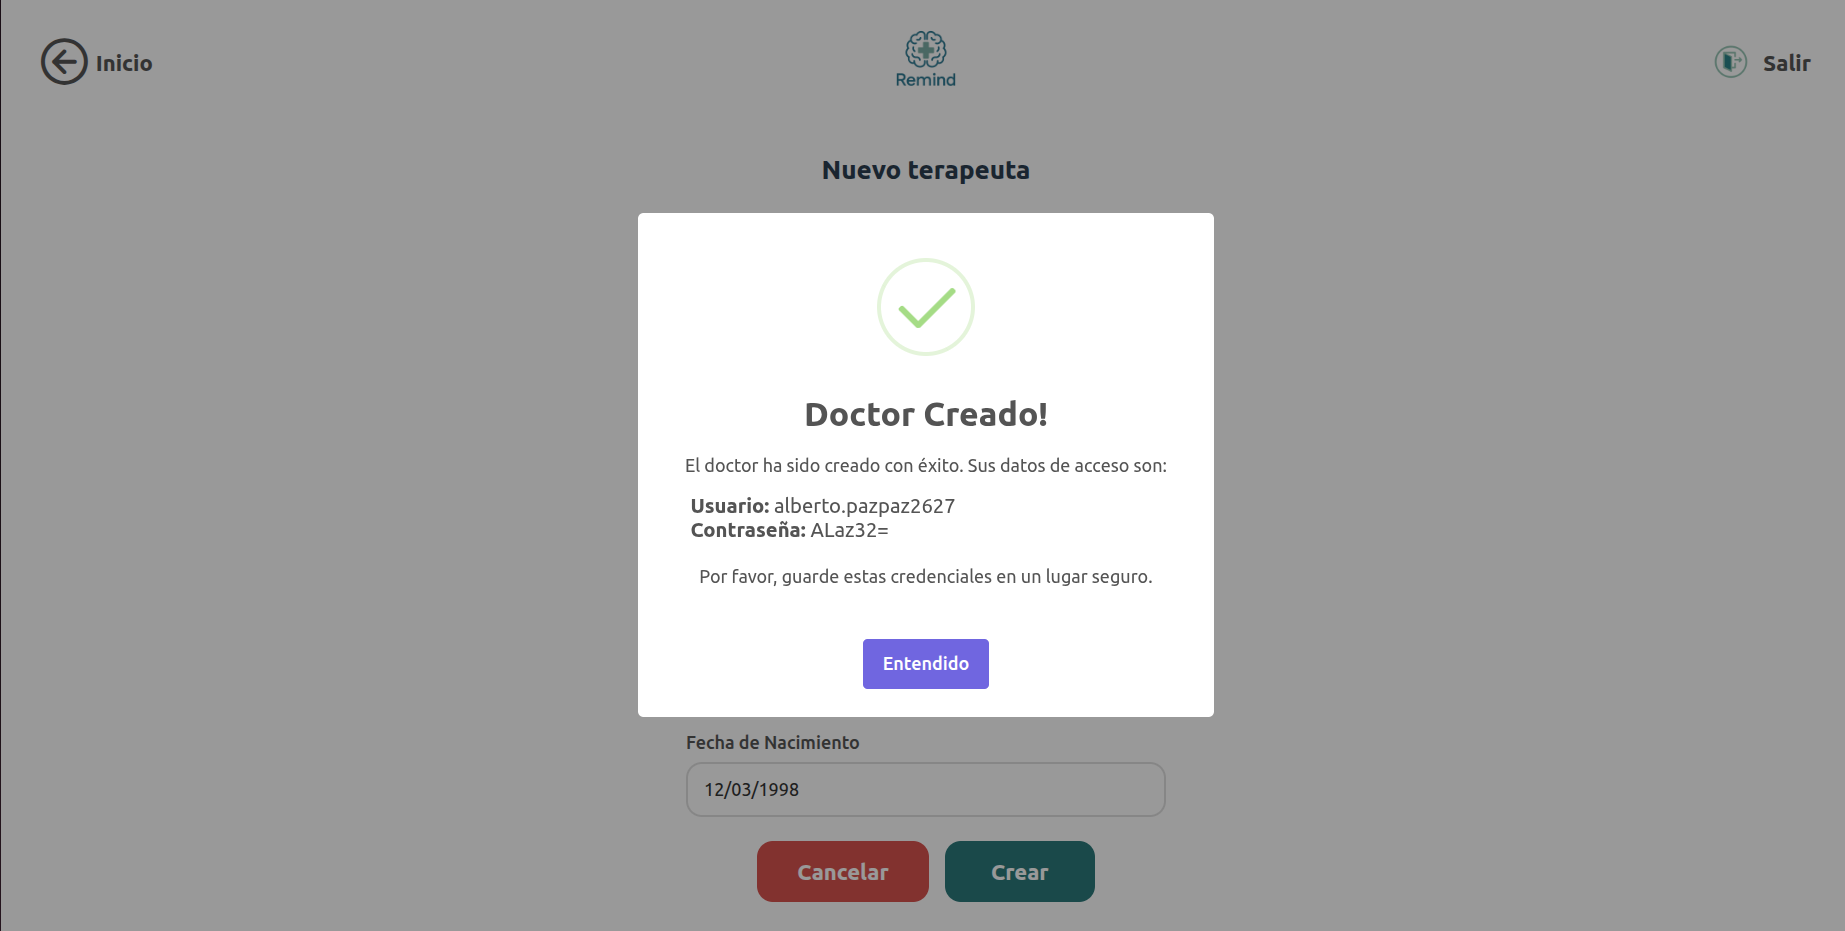
\includegraphics[width=\textwidth]{imagenes/manual/credenciales.png}
    \caption{Credenciales del nuevo terapeuta}
\end{figure}

\begin{center}
    \fbox{\parbox{0.9\textwidth}{\textbf{Nota importante:} Anote estas credenciales y entréguelas al terapeuta. No podrá volver a ver la contraseña generada, aunque sí podrá generar una nueva más adelante.}}
\end{center}

\subsection{Acciones sobre un terapeuta}

Cada terapeuta en el listado dispone de cuatro botones con las siguientes funciones:

\begin{itemize}
    \item \textbf{Lápiz (Editar):} pulsa este botón para modificar los datos del terapeuta. Se abrirá un formulario con la información actual para que pueda actualizarla.
    \item \textbf{Llave (Ver usuario):} pulsa este botón para consultar el nombre de usuario del terapeuta.
    \item \textbf{Rueda (Restablecer contraseña):} si el terapeuta ha olvidado su contraseña, este botón genera una nueva y la muestra en pantalla.
    \item \textbf{Papelera (Eliminar):} pulsa este botón para eliminar al terapeuta del sistema. La aplicación le pedirá confirmación antes de borrar los datos.
\end{itemize}

\section{Terapeuta}

El terapeuta es el profesional sanitario que trabaja directamente con los pacientes. Puede gestionar sus perfiles, asignarles juegos de estimulación cognitiva y realizar un seguimiento de su progreso.

\begin{figure}[H]
    \centering
    
\includegraphics[width=\textwidth]{imagenes/manual/home_doctor.png}
    \caption{Pantalla principal del terapeuta}
\end{figure}

Desde el menú deslizable puede acceder a las distintas secciones: \textbf{Pacientes}, \textbf{Agendas} y \textbf{Seguimiento}.

\begin{figure}[H]
    \centering
    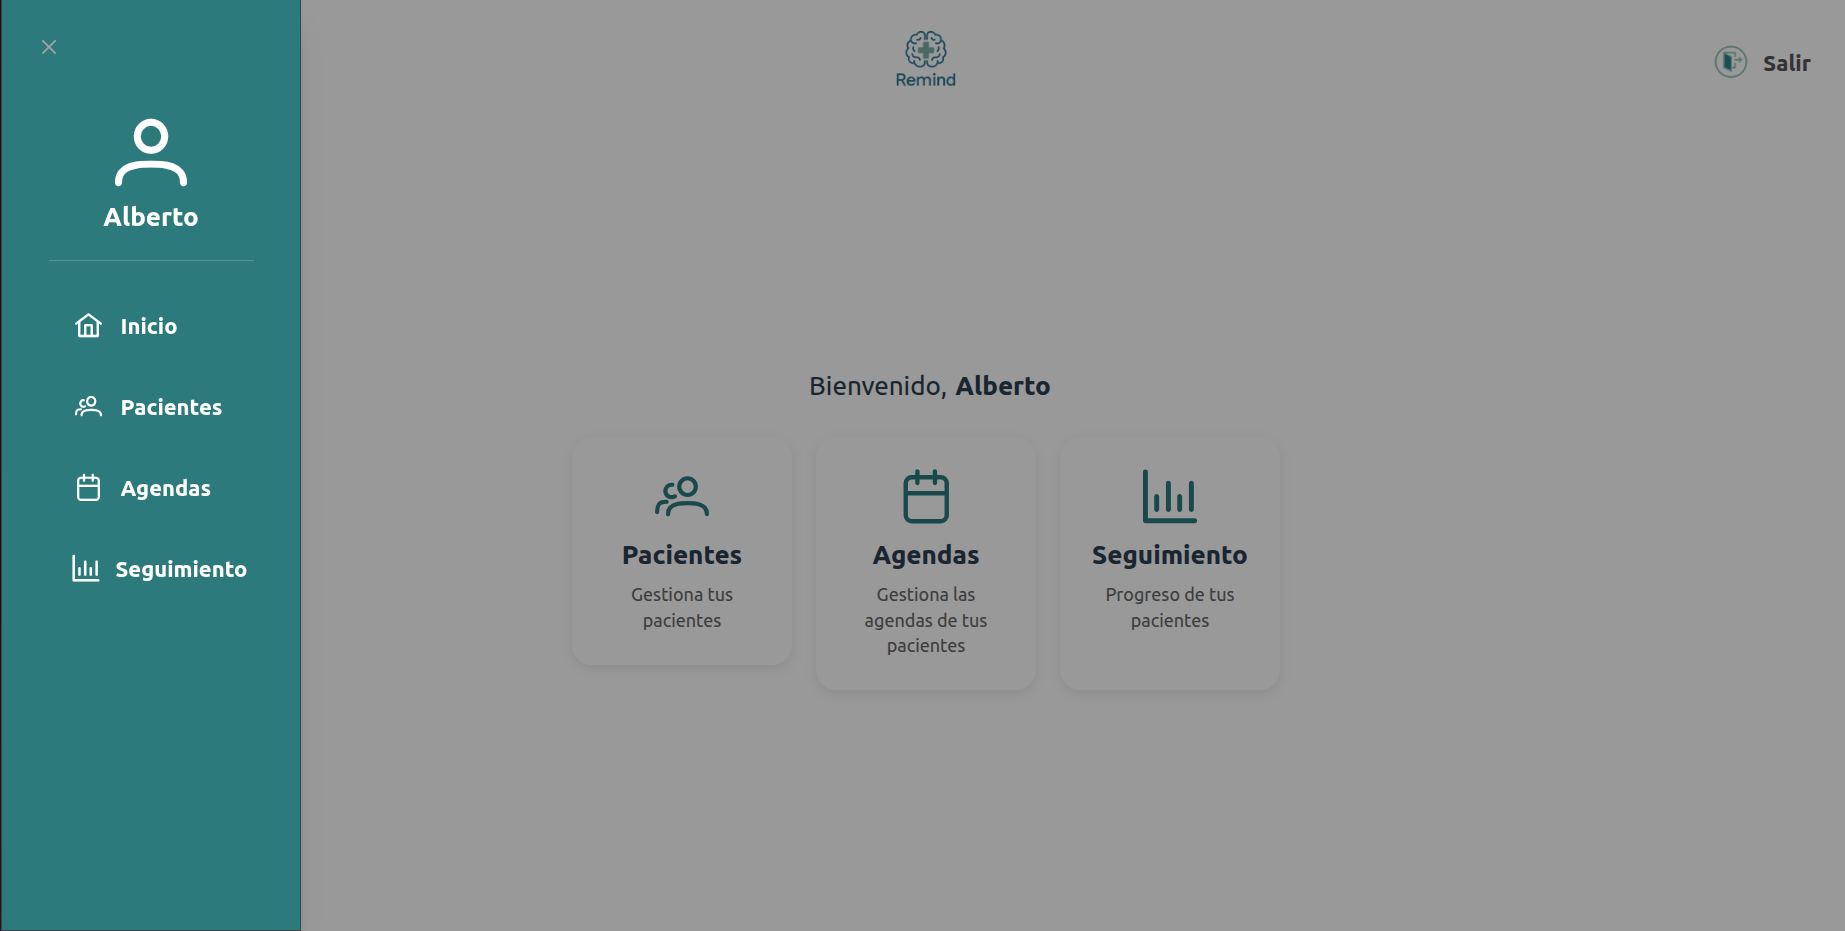
\includegraphics[width=\textwidth]{imagenes/manual/menu_doctor.png}
    \caption{Menú de navegación del terapeuta}
\end{figure}

\subsection{Gestión de pacientes}

En la sección \textbf{Pacientes} se muestra un listado con todos los pacientes asignados al terapeuta.

\begin{figure}[H]
    \centering
    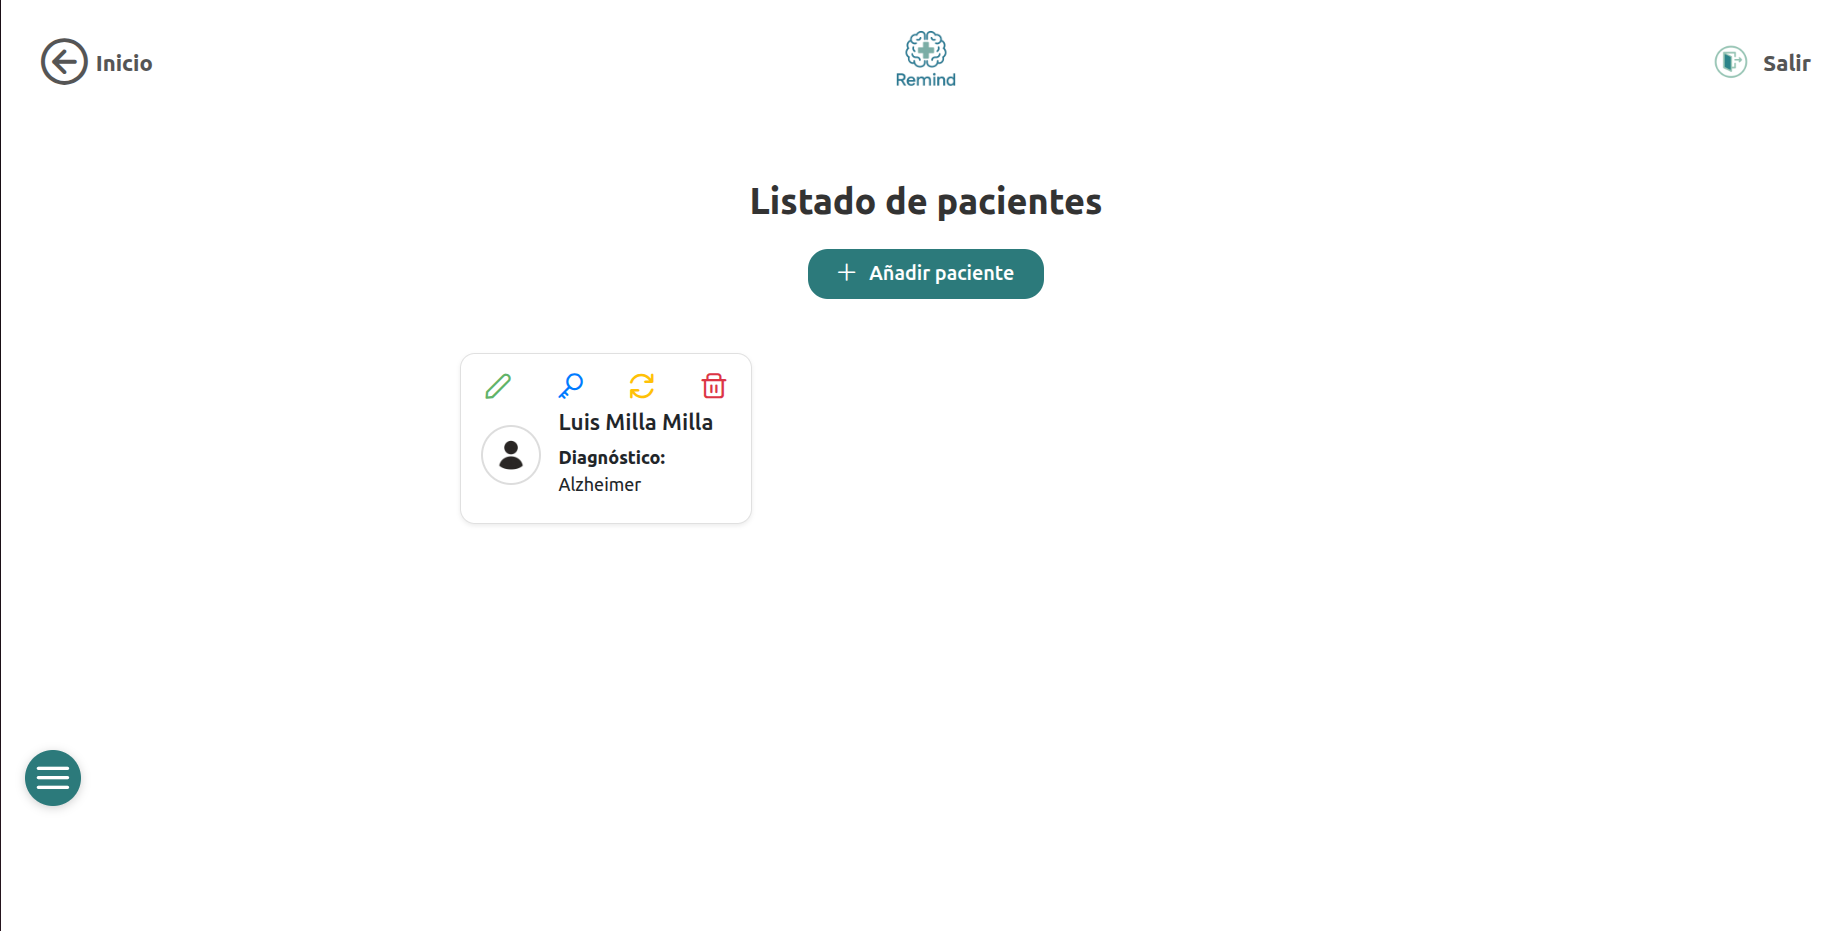
\includegraphics[width=\textwidth]{imagenes/manual/listado_pacie.png}
    \caption{Listado de pacientes del terapeuta}
\end{figure}

\subsubsection{Crear un paciente}

Pulse el botón \textbf{Añadir paciente} y rellene el formulario con sus datos: nombre, apellidos, información de contacto y datos del cuidador si lo hubiera. La aplicación generará automáticamente las credenciales del paciente.

\subsubsection{Acciones sobre un paciente}

Al igual que con los terapeutas, cada paciente dispone de botones para:

\begin{itemize}
    \item \textbf{Editar} sus datos personales.
    \item \textbf{Ver nombre de usuario} pulsando el icono de la llave.
    \begin{figure}[H]
        \centering
        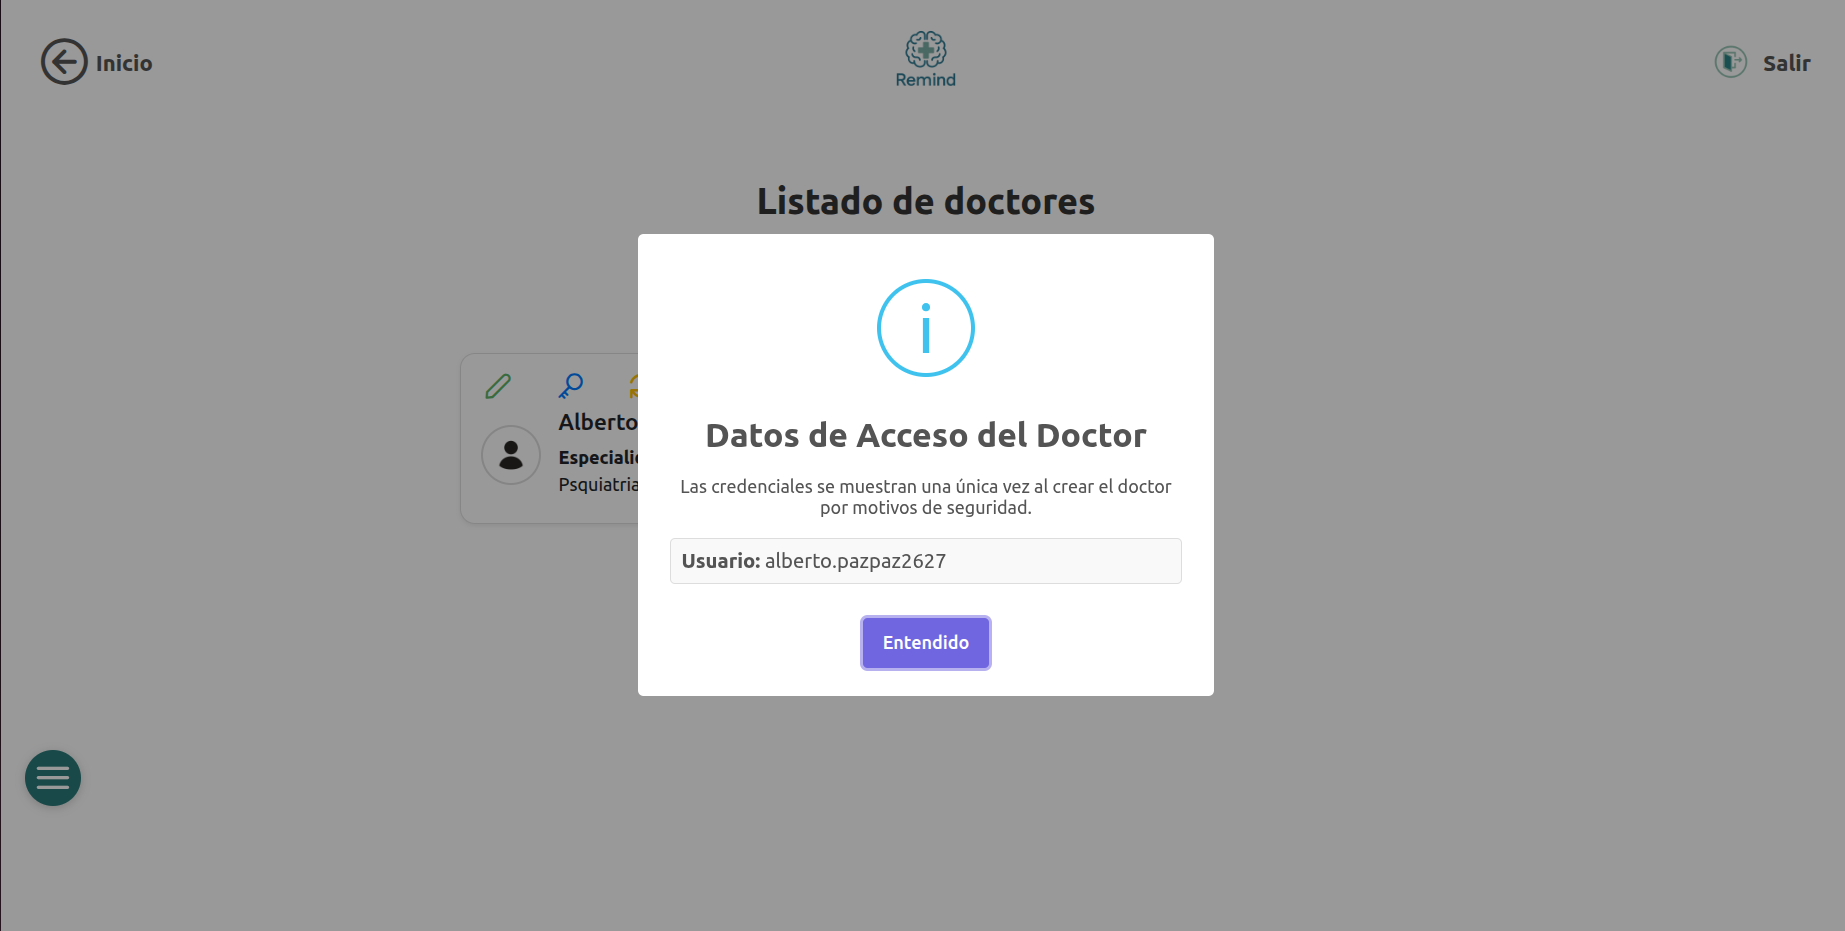
\includegraphics[width=\textwidth]{imagenes/manual/credencial_usuario.png}
        \caption{Consulta del nombre de usuario de un paciente}
    \end{figure}
    \item \textbf{Restablecer la contraseña} si el paciente la olvida.
    \begin{figure}[H]
        \centering
        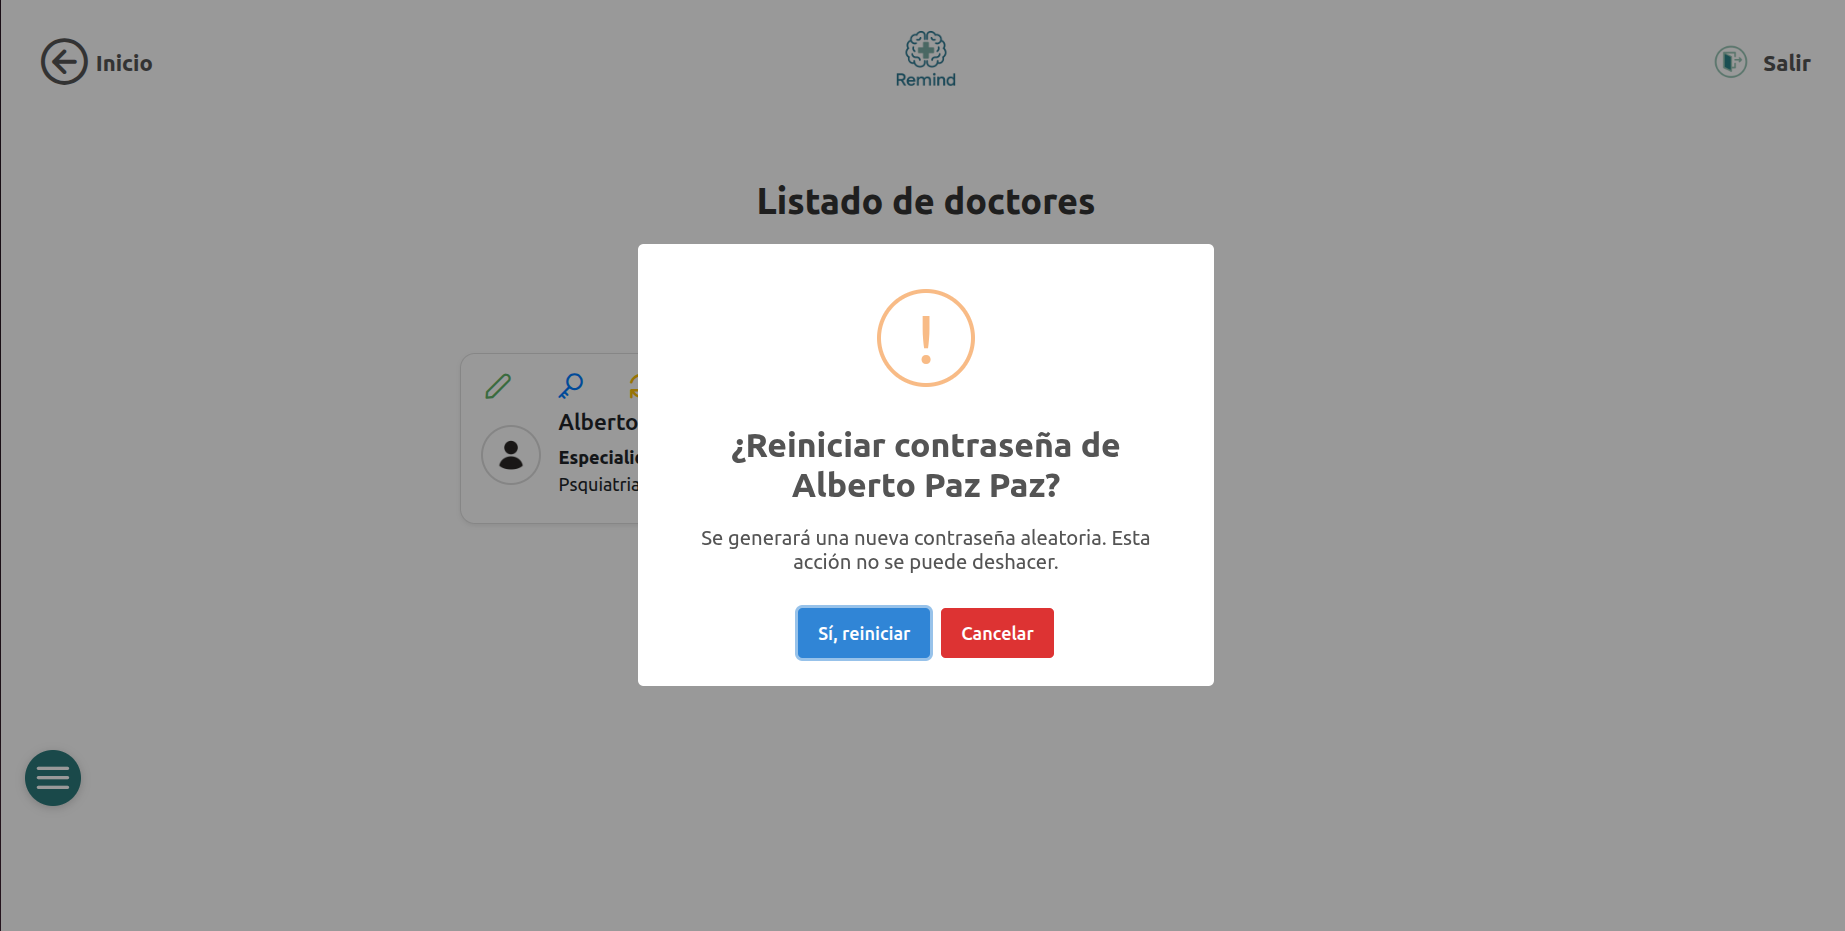
\includegraphics[width=\textwidth]{imagenes/manual/reseteo_credenciales.png}
        \caption{Restablecimiento de contraseña de un paciente}
    \end{figure}
    \item \textbf{Eliminar} al paciente del sistema, con confirmación previa.
    \begin{figure}[H]
        \centering
        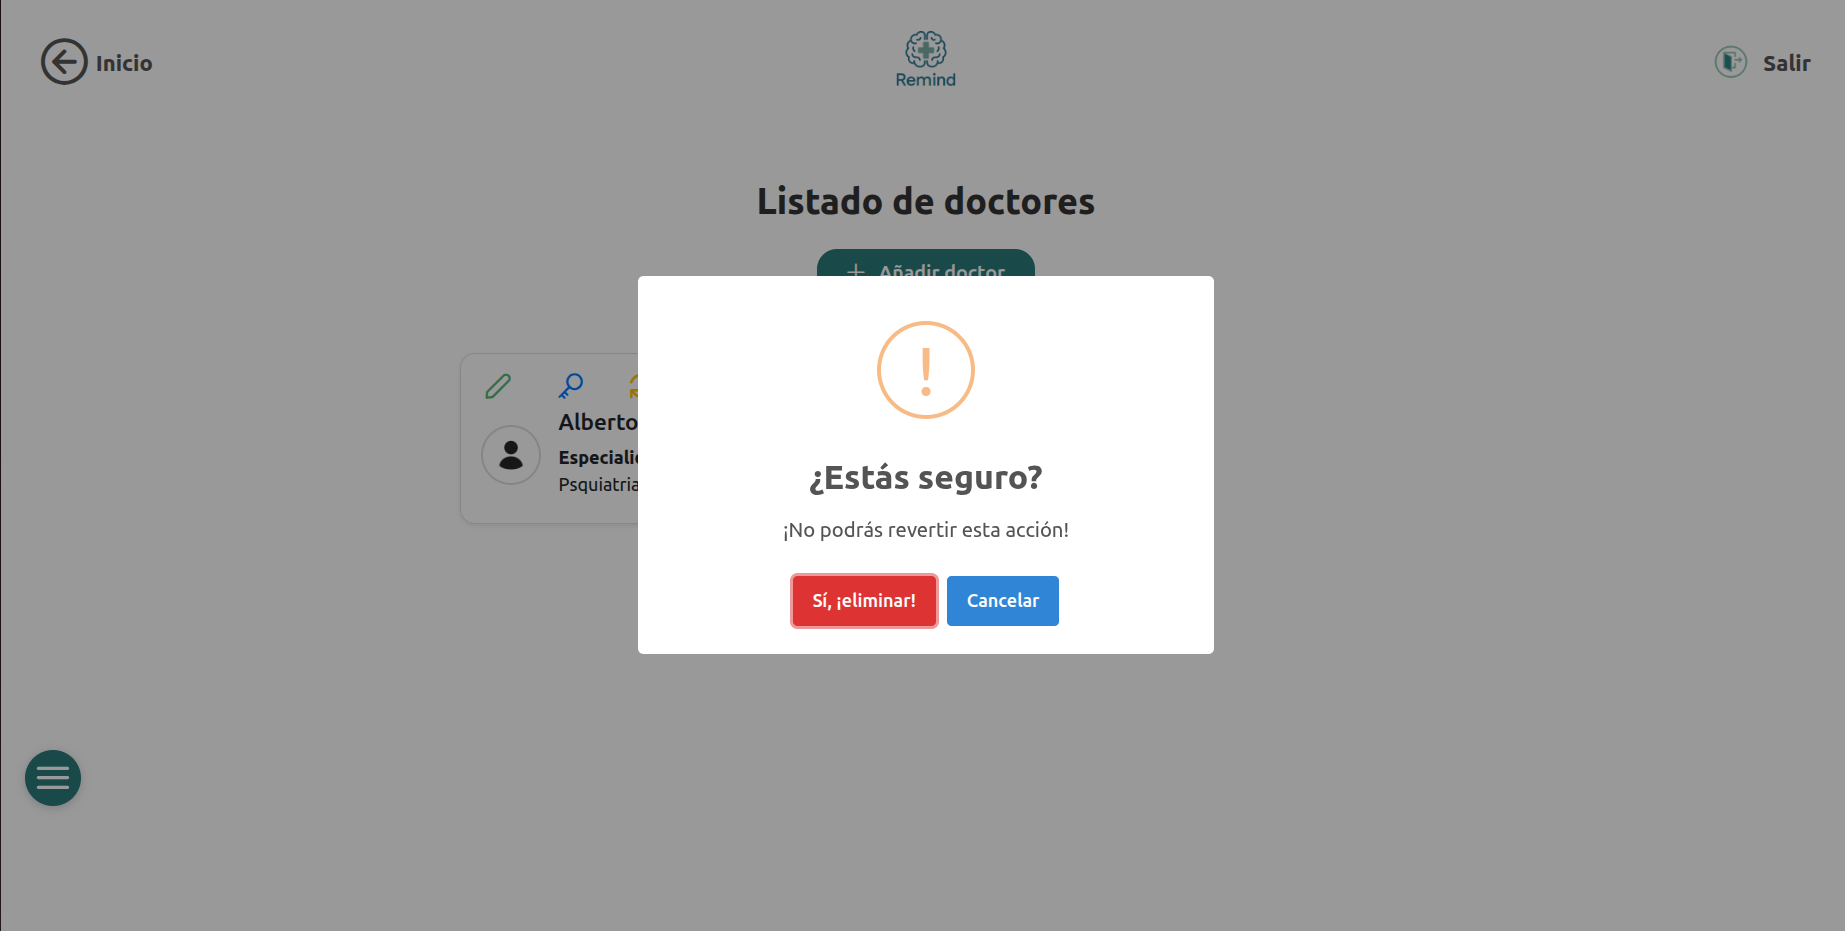
\includegraphics[width=\textwidth]{imagenes/manual/eliminar_usuario.png}
        \caption{Eliminación de un paciente}
    \end{figure}
\end{itemize}

\subsection{Gestión de agendas: asignar juegos a un paciente}

Cada paciente tiene una agenda personal donde el terapeuta asigna los juegos que debe realizar. Para acceder, vaya a la sección \textbf{Agendas} desde el menú.

\begin{figure}[H]
    \centering
    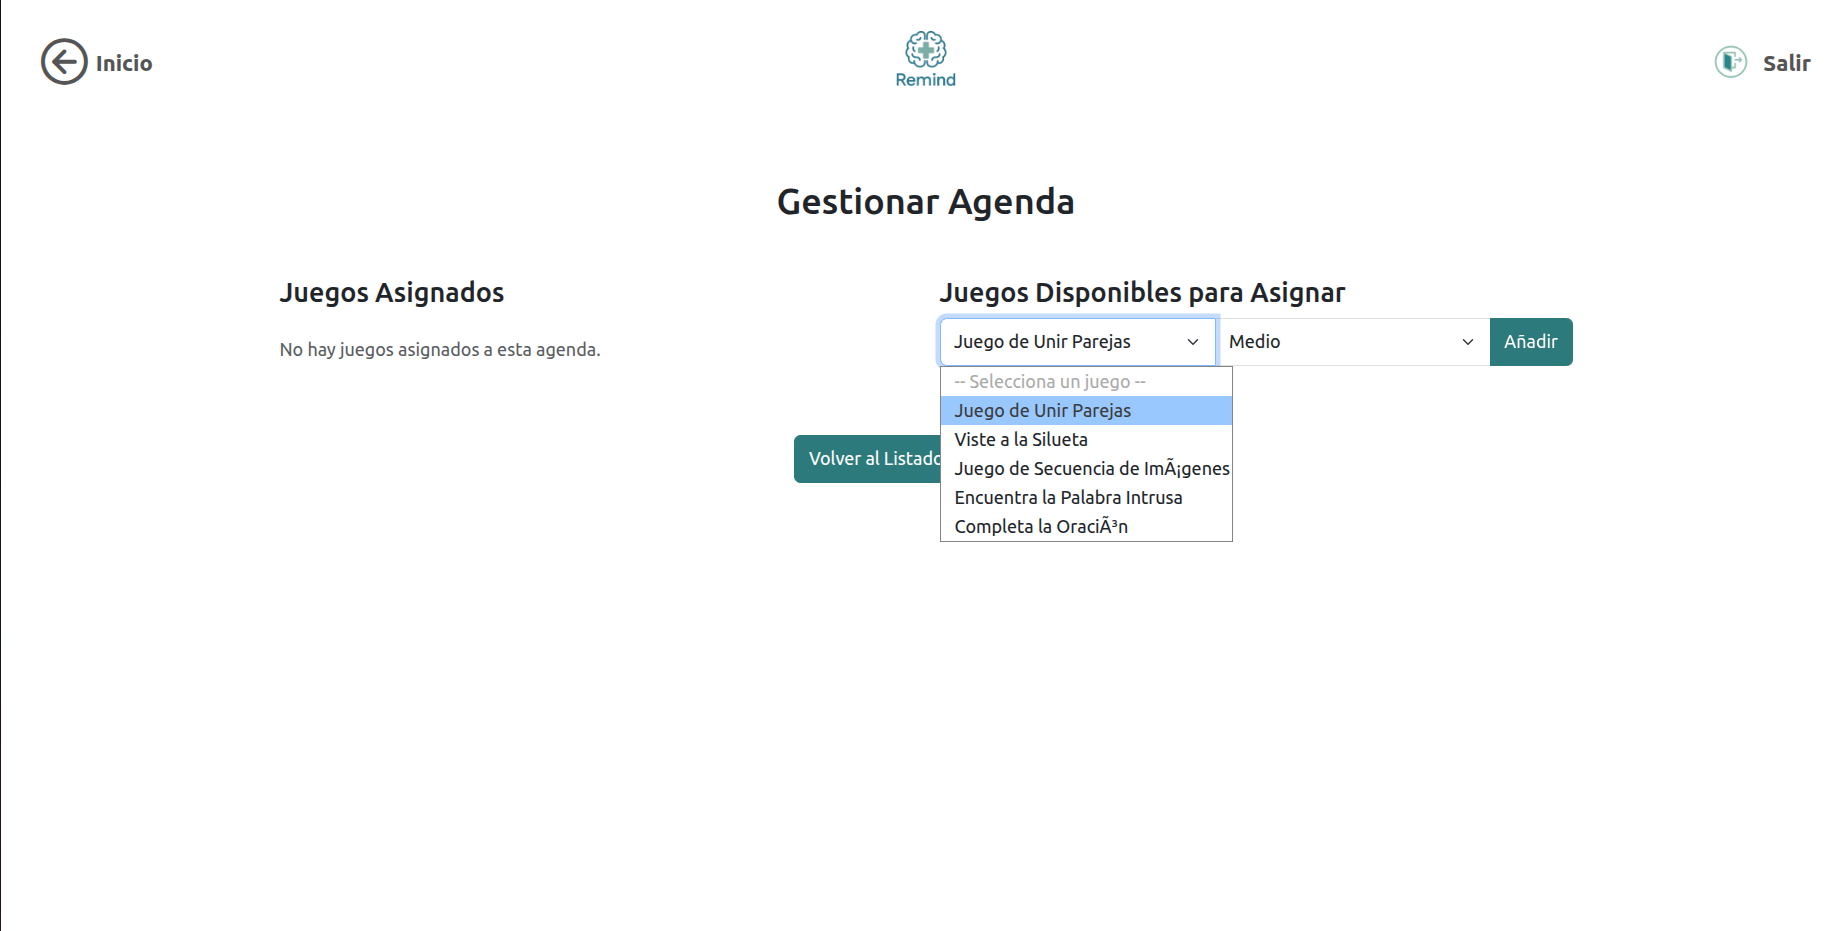
\includegraphics[width=\textwidth]{imagenes/manual/asignar_juego.png}
    \caption{Asignación de juegos a un paciente}
\end{figure}

Para asignar un juego:

\begin{enumerate}
    \item Seleccione el \textbf{juego} que desea asignar del menú desplegable.
    \item Elija el \textbf{nivel de dificultad}:
    \begin{itemize}
        \item \textbf{Fácil (nivel 1):} menos elementos y tareas más sencillas. Recomendado para las primeras sesiones o para pacientes con deterioro cognitivo moderado.
        \item \textbf{Media (nivel 2):} número moderado de elementos. Adecuado para pacientes que ya han practicado.
        \item \textbf{Difícil (nivel 3):} máximo número de elementos y mayor complejidad. Para pacientes con buen rendimiento cognitivo.
    \end{itemize}
    \item Pulse el botón \textbf{Añadir} para incluir el juego en la agenda del paciente.
\end{enumerate}

Los juegos asignados aparecerán en la parte inferior con su nivel de dificultad. Puede eliminarlos pulsando el icono de la papelera.

\subsection{Seguimiento del progreso}

La sección de \textbf{Seguimiento} permite al terapeuta consultar el avance de cada paciente de forma visual.

\begin{figure}[H]
    \centering
    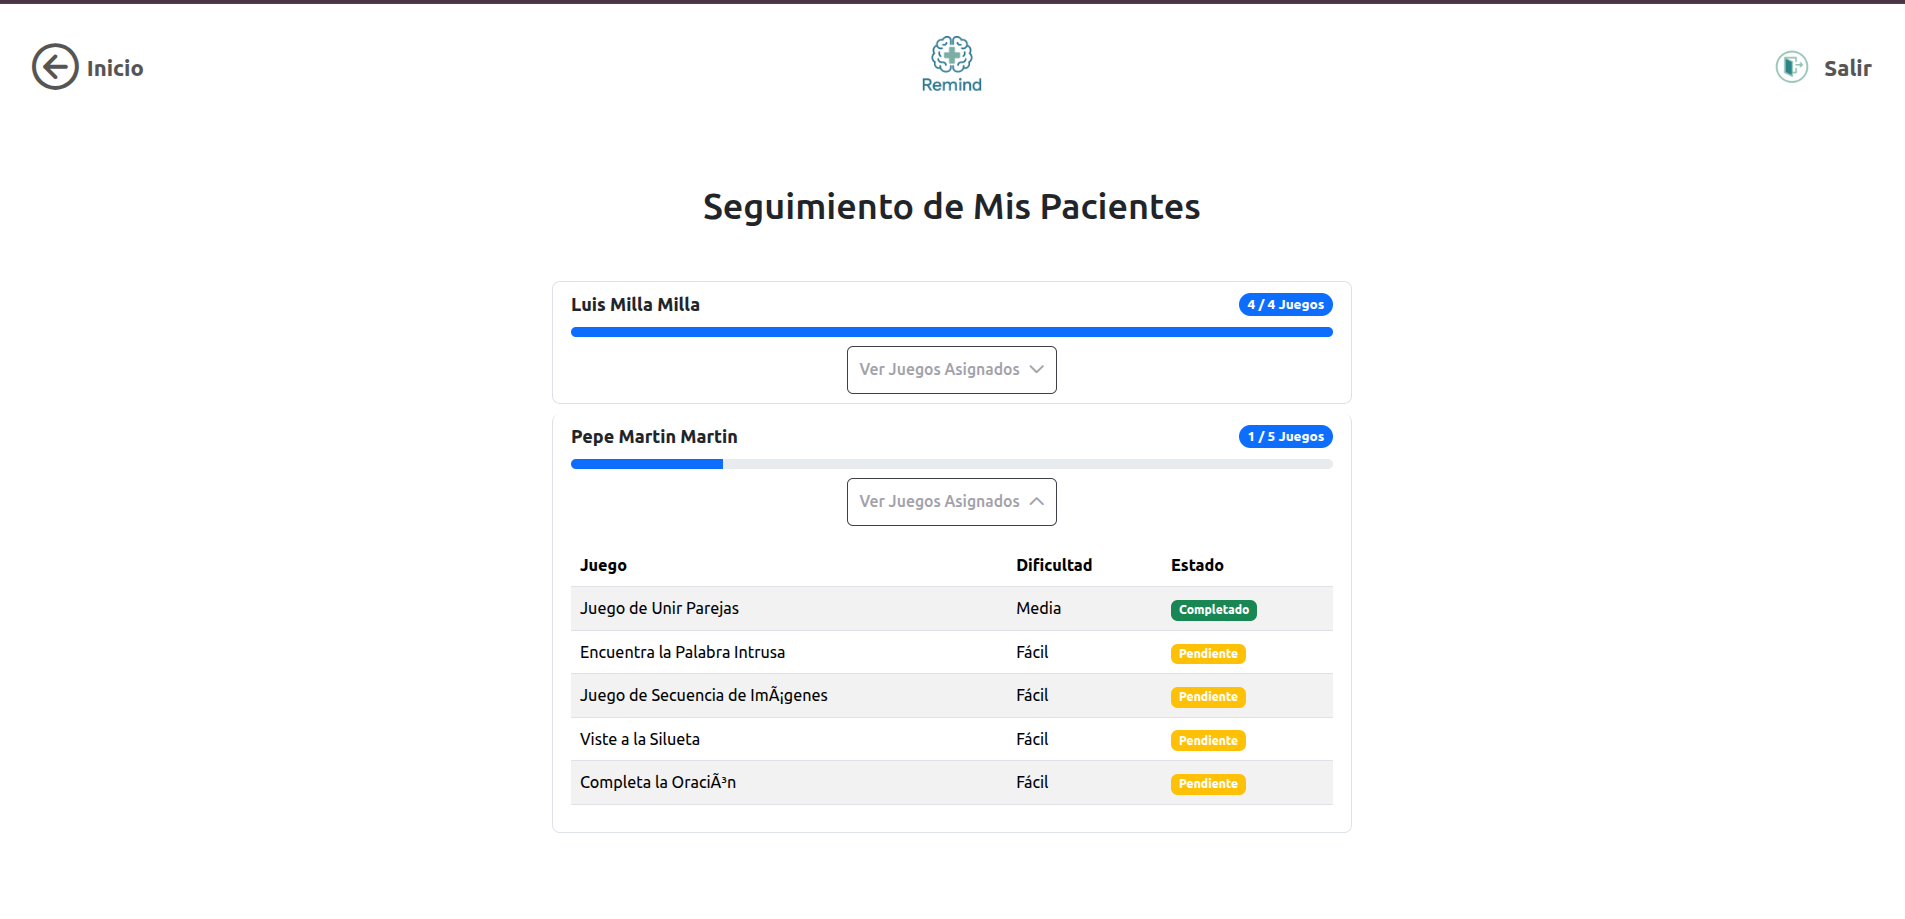
\includegraphics[width=\textwidth]{imagenes/manual/seguimiento_pacientes.png}
    \caption{Seguimiento del progreso de los pacientes}
\end{figure}

Para cada paciente se muestra:

\begin{itemize}
    \item \textbf{Nombre completo} del paciente.
    \item \textbf{Progreso general} indicado como ``X / Y juegos completados''.
    \item \textbf{Barra de progreso} que representa visualmente el porcentaje completado.
    \item Al desplegar la sección \textbf{Ver juegos asignados}, se muestra una tabla detallada con:
    \begin{itemize}
        \item \textbf{Juego:} nombre del juego asignado.
        \item \textbf{Dificultad:} fácil, media o difícil.
        \item \textbf{Estado:} completado (marcado en verde) o pendiente (marcado en amarillo).
    \end{itemize}
\end{itemize}

Esta vista permite identificar rápidamente qué pacientes necesitan más atención y qué juegos están pendientes de realizar.

\section{El paciente}

El paciente es la persona que realiza los juegos de estimulación cognitiva. Su interfaz está diseñada para ser sencilla y accesible, con botones grandes e instrucciones claras.

\subsection{Pantalla principal del paciente}

Al iniciar sesión, el paciente accede a su pantalla principal donde se muestran sus \textbf{logros} y el \textbf{acceso a los juegos}.

\begin{figure}[H]
    \centering
    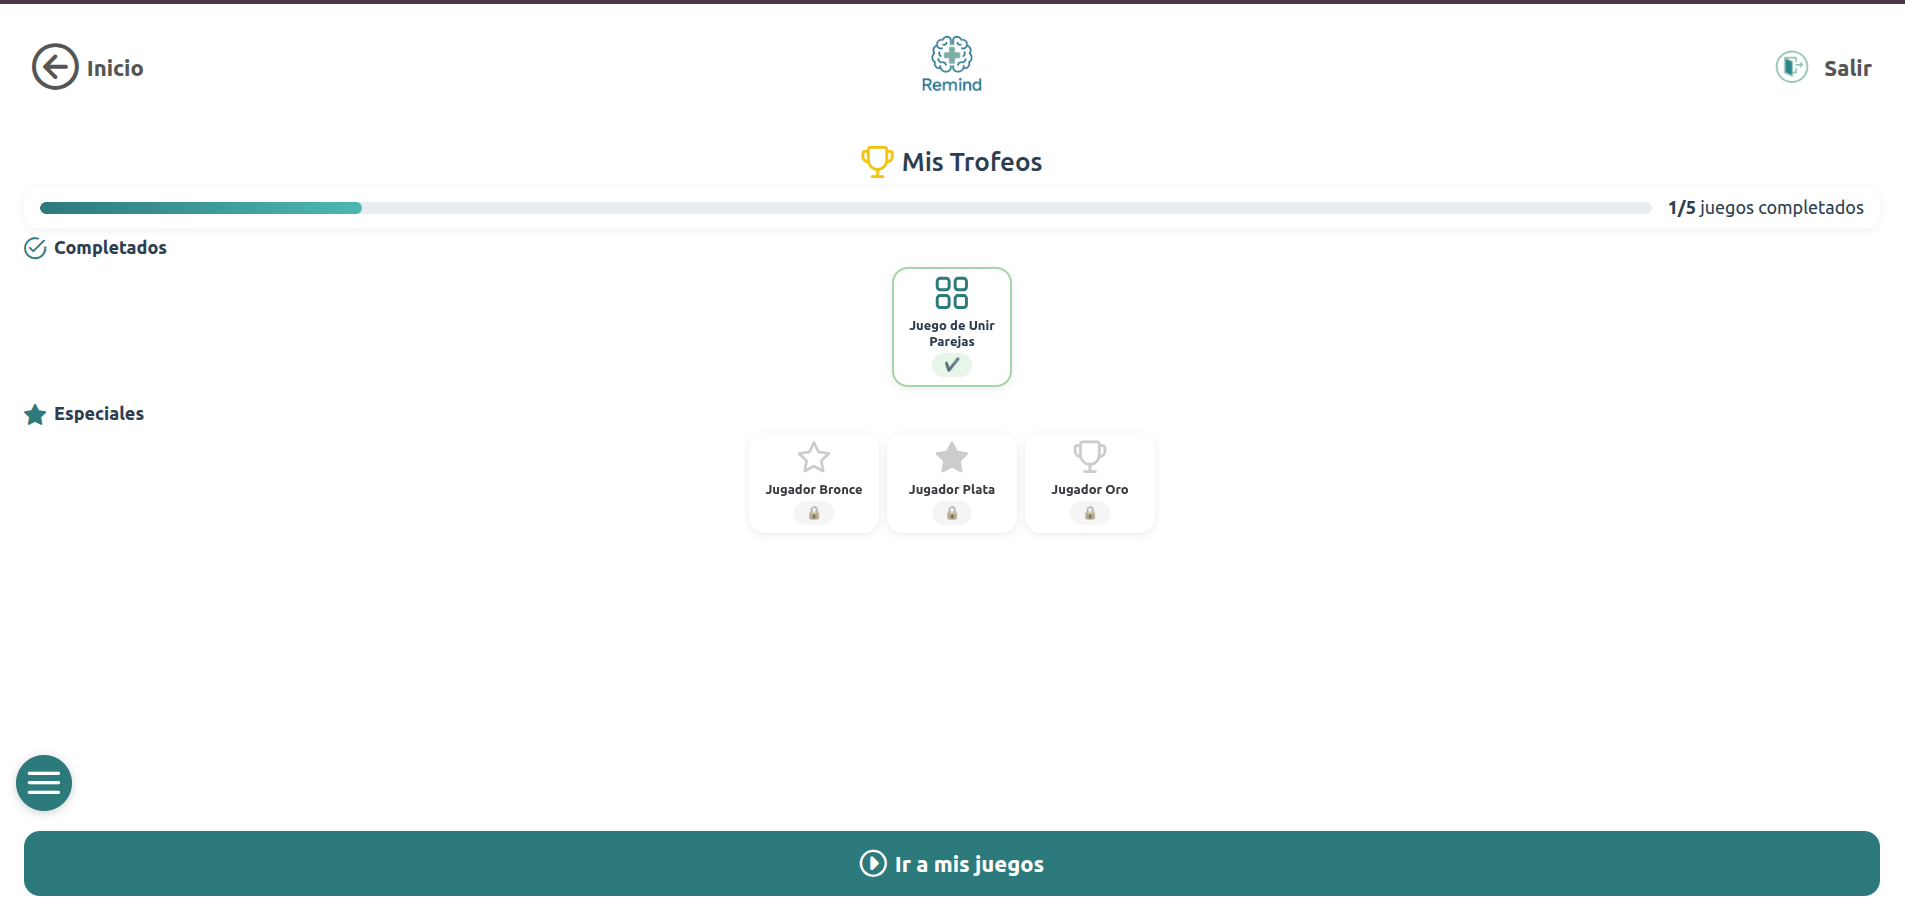
\includegraphics[width=\textwidth]{imagenes/manual/home_paciente.png}
    \caption{Pantalla principal del paciente}
\end{figure}

En esta pantalla aparece:

\begin{itemize}
    \item \textbf{Barra de progreso:} indica cuántos juegos ha completado de los que tiene asignados (por ejemplo, ``2 / 4 juegos completados'').
    \item \textbf{Sección ``Mis Trofeos'':} muestra los juegos que ya ha completado con un icono distintivo. También incluye medallas especiales por alcanzar hitos:
    \begin{itemize}
        \item \textbf{Bronce:} al completar 3 juegos distintos.
        \item \textbf{Plata:} al completar 5 juegos distintos.
        \item \textbf{Oro:} al completar los 6 juegos disponibles.
    \end{itemize}
    \item \textbf{Botón ``Ir a mis juegos'':} pulsa este botón para ver los juegos pendientes y empezar a jugar.
\end{itemize}

\subsection{Agenda de juegos del paciente}

Al pulsar \textbf{Ir a mis juegos}, el paciente accede a su agenda personal. Esta pantalla se divide en dos secciones:

\begin{figure}[H]
    \centering
    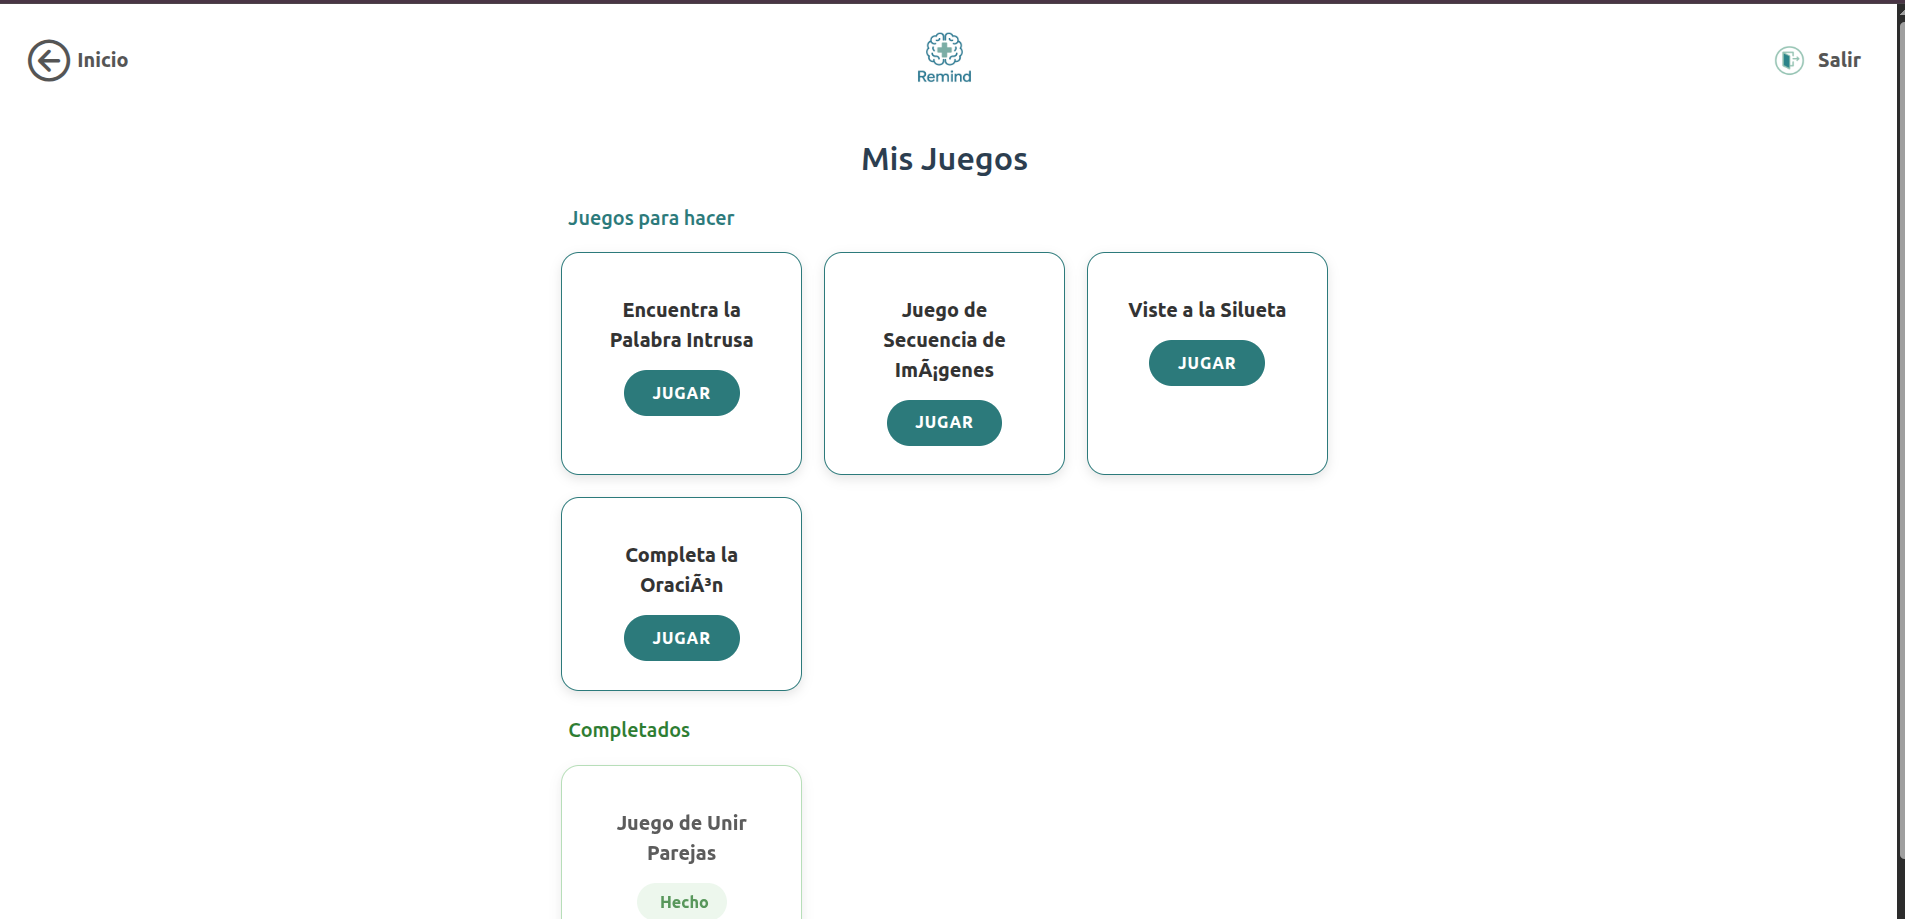
\includegraphics[width=\textwidth]{imagenes/manual/tareas_paciente.png}
    \caption{Agenda de juegos del paciente}
\end{figure}

\begin{itemize}
    \item \textbf{Juegos para hacer:} muestra los juegos que el terapeuta le ha asignado y que aún no ha realizado. Cada juego aparece como una tarjeta con su nombre y un botón \textbf{Jugar}.
    \item \textbf{Completados:} muestra los juegos que ya ha finalizado, marcados con un icono de verificación.
\end{itemize}

Para empezar a jugar, pulse el botón \textbf{Jugar} en el juego que desee realizar.

\subsection{Cómo se juega}

Cada juego comienza mostrando una breve historia o contexto que explica la actividad de forma amena, lo que ayuda a reducir la sensación de estar siendo evaluado.

\subsubsection{Instrucciones en pantalla}

Al empezar cada juego, el paciente ve una cabecera con el nombre del juego y un botón \textbf{Instrucciones}. Al pulsarlo, se abre una ventana emergente (modal) que explica cómo se juega.

\begin{figure}[H]
    \centering
    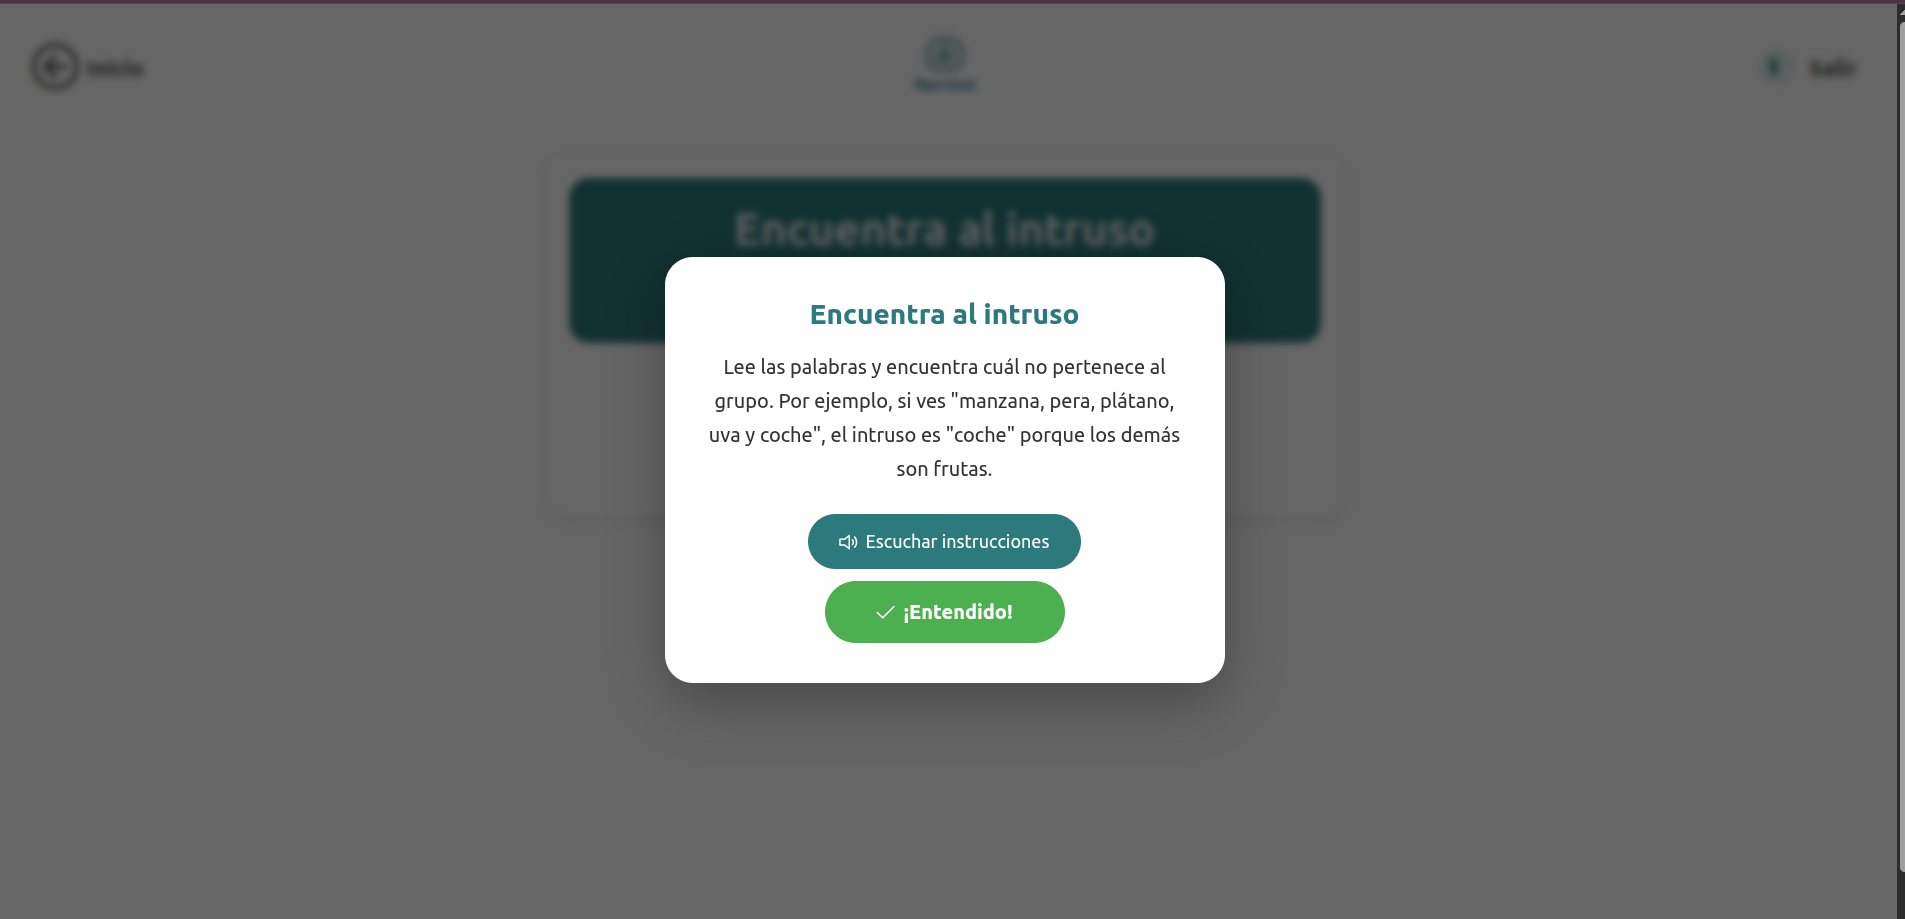
\includegraphics[width=\textwidth]{imagenes/manual/instrucciones.png}
    \caption{Ejemplo del modal de instrucciones común a todos los juegos}
\end{figure}

Este modal incluye:

\begin{itemize}
    \item El \textbf{título} del juego.
    \item El \textbf{texto explicativo} con las reglas, escrito en letra grande y clara.
    \item Un botón \textbf{Escuchar instrucciones} con forma de altavoz que reproduce las normas en audio. Especialmente útil para pacientes con dificultades de lectura o visión reducida.
    \item Un botón \textbf{¡Entendido!} para cerrar la ventana y comenzar a jugar.
\end{itemize}

El paciente puede volver a abrir el modal pulsando el botón \textbf{Instrucciones} en cualquier momento durante la partida. El botón de audio también puede pulsarse tantas veces como sea necesario.

\subsubsection{Interacción durante el juego}

El paciente interactúa mediante \textbf{pulsaciones} (tocar un elemento en la pantalla) o \textbf{arrastrar y soltar} (mover un elemento de un lugar a otro). No se necesita usar el teclado ni el ratón de forma avanzada; todo se hace con el dedo en una pantalla táctil o con el botón izquierdo del ratón.

\subsubsection{Qué ocurre al completar un juego}

Cuando el paciente termina un juego correctamente, aparece una pantalla de felicitación y la aplicación lo marca como completado en su agenda.

\begin{figure}[H]
    \centering
    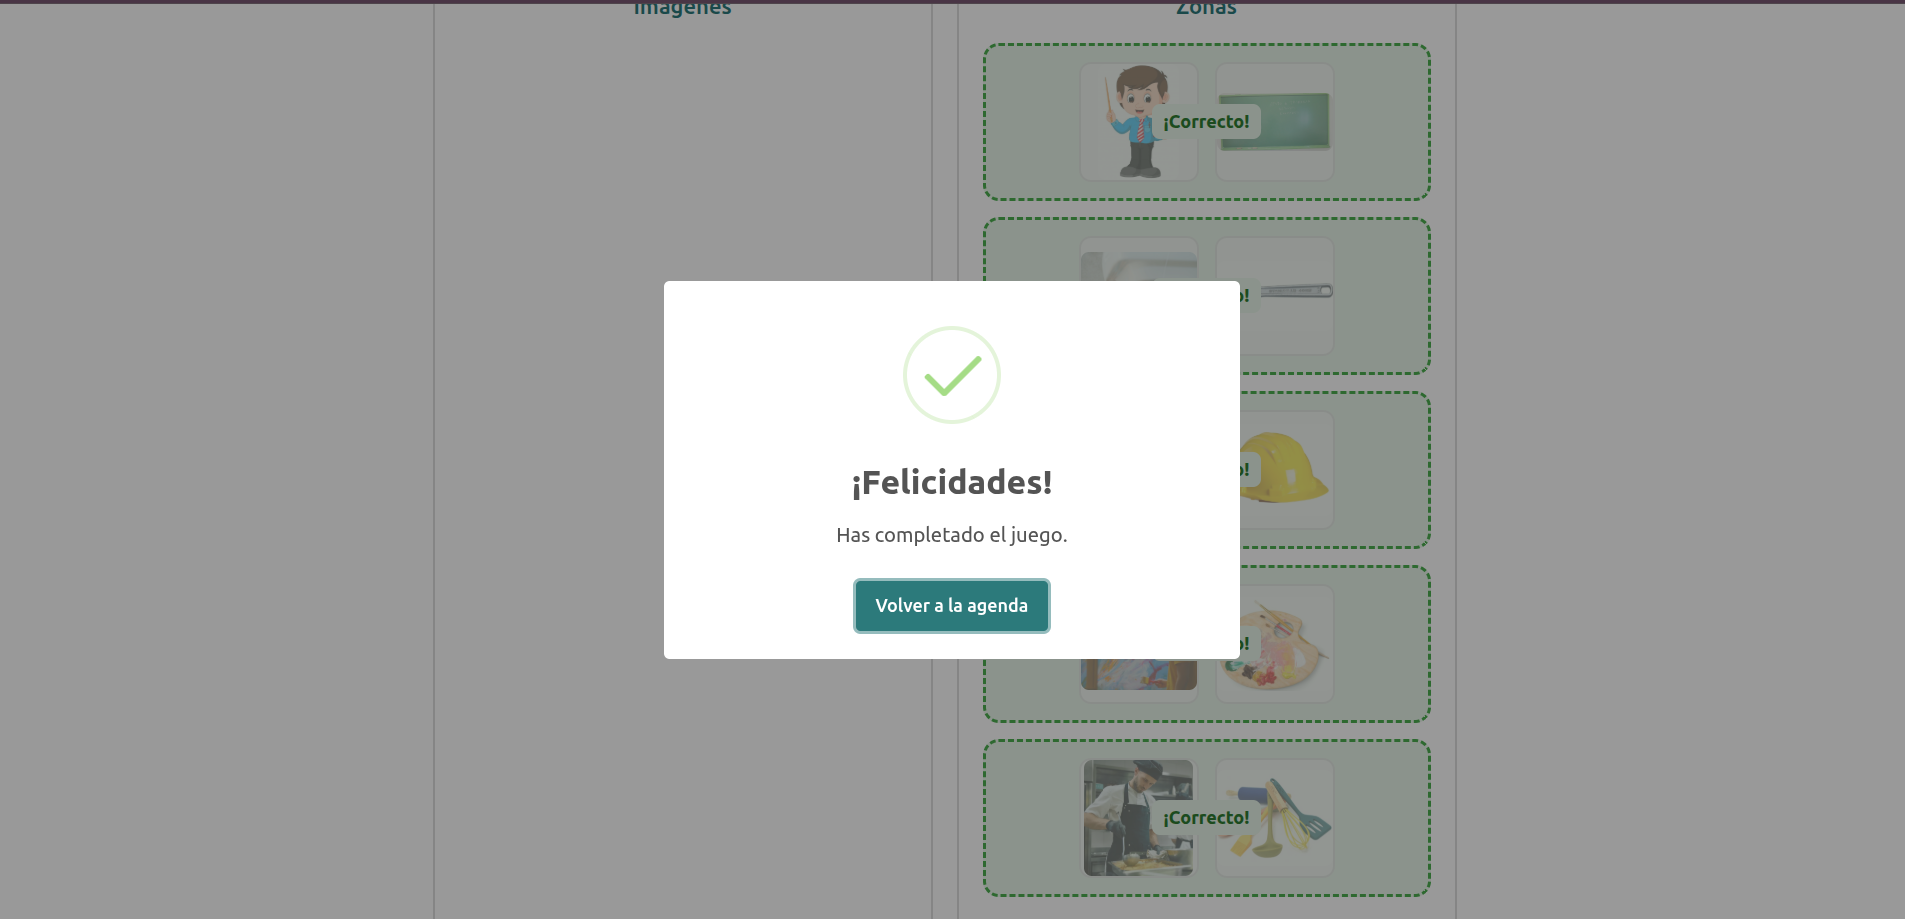
\includegraphics[width=\textwidth]{imagenes/manual/juego_completado.png}
    \caption{Pantalla de juego completado}
\end{figure}

\begin{center}
    \fbox{\parbox{0.9\textwidth}{\textbf{Consejo:} Si el paciente se siente frustrado o se equivoca, puede pulsar el botón \textbf{Reiniciar} para volver a empezar el juego desde el principio.}}
\end{center}

\section{Los juegos de estimulación cognitiva}

ReMind incluye seis juegos diseñados para trabajar diferentes capacidades cognitivas: memoria, atención, lenguaje, razonamiento y cálculo.

\subsection{Ordenar la secuencia}

\begin{itemize}
    \item \textbf{Qué trabaja:} memoria visual y capacidad de ordenación temporal.
    \item \textbf{Instrucciones en audio:} sí.
    \item \textbf{Cómo se juega:} aparece una secuencia de imágenes que se muestran una a una. Después, las imágenes se ocultan y el paciente debe pulsarlas en el mismo orden en que aparecieron.
    \item \textbf{Dificultad:} nivel fácil (4 imágenes), medio (5 imágenes), difícil (6 imágenes).
\end{itemize}

\begin{figure}[H]
    \centering
    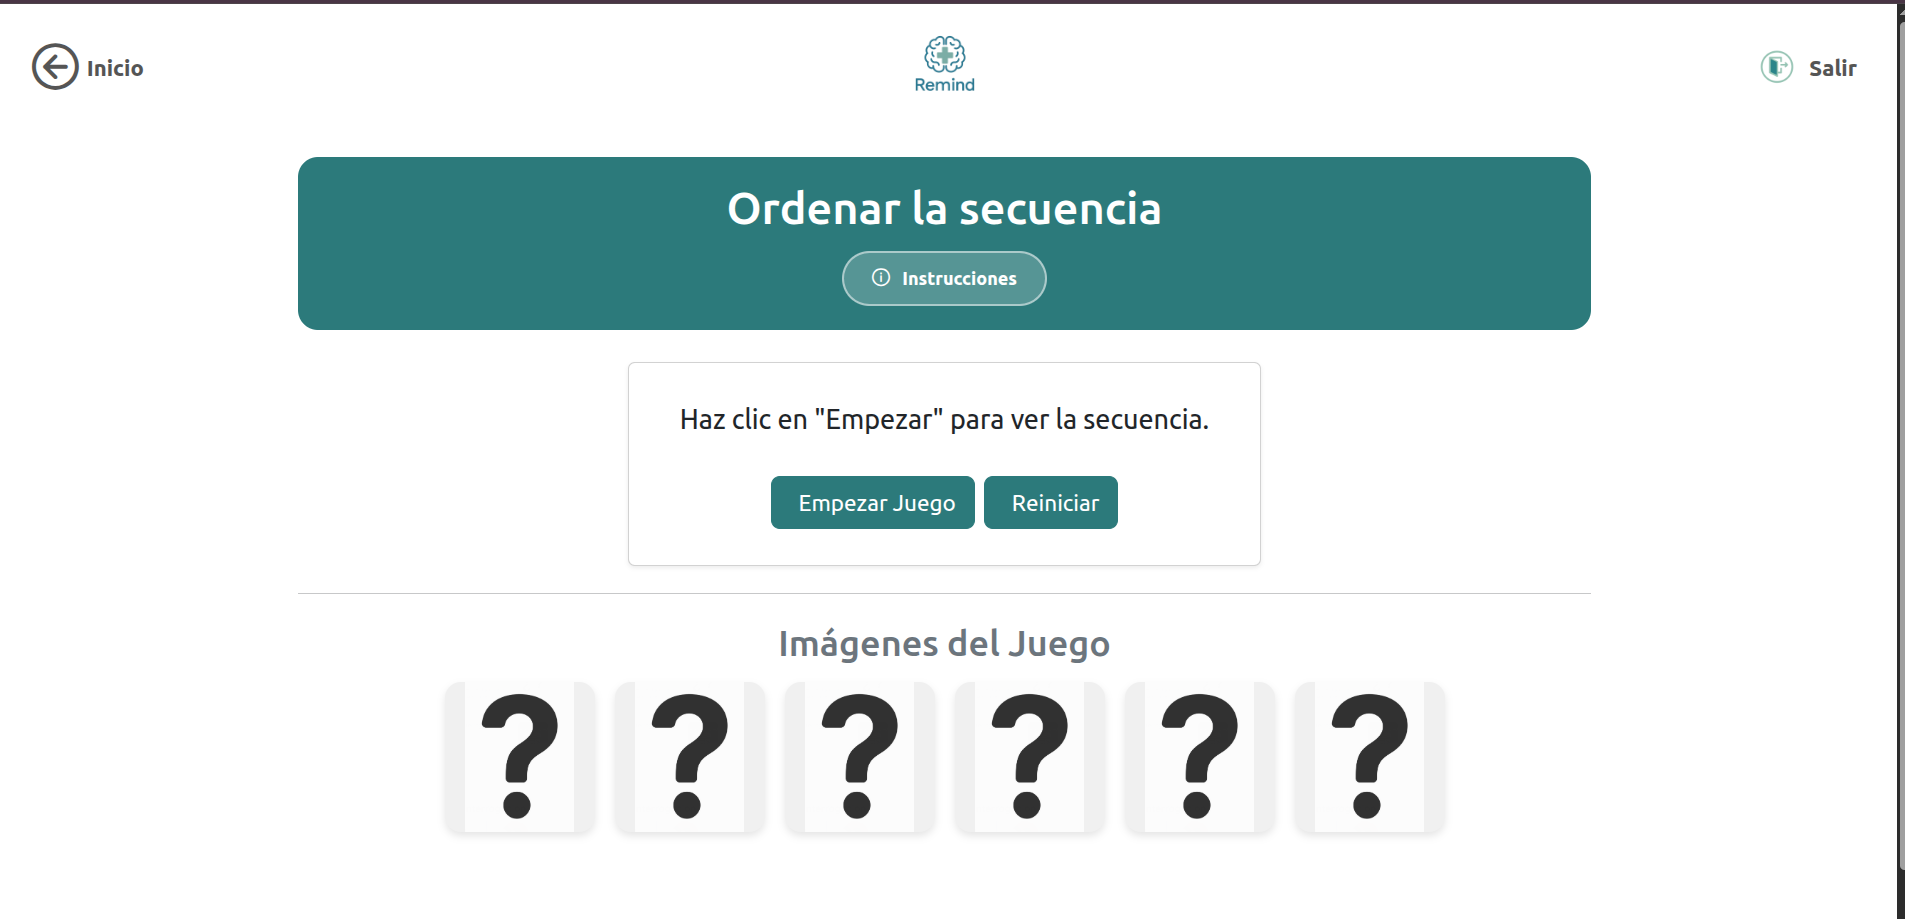
\includegraphics[width=\textwidth]{imagenes/manual/juego_secuencia.png}
    \caption{Juego ``Ordenar la secuencia''}
\end{figure}

\subsection{Relacionar objetos y profesiones}

\begin{itemize}
    \item \textbf{Qué trabaja:} asociación semántica y categorización.
    \item \textbf{Instrucciones en audio:} sí.
    \item \textbf{Cómo se juega:} en un mercado, las herramientas de los oficios se han mezclado. El paciente debe arrastrar cada objeto y colocarlo junto con la profesión correspondiente (por ejemplo, el casco con el constructor, el termómetro con la médica).
    \item \textbf{Dificultad:} nivel fácil (4 parejas), medio (5 parejas), difícil (6 parejas).
\end{itemize}

\begin{figure}[H]
    \centering
    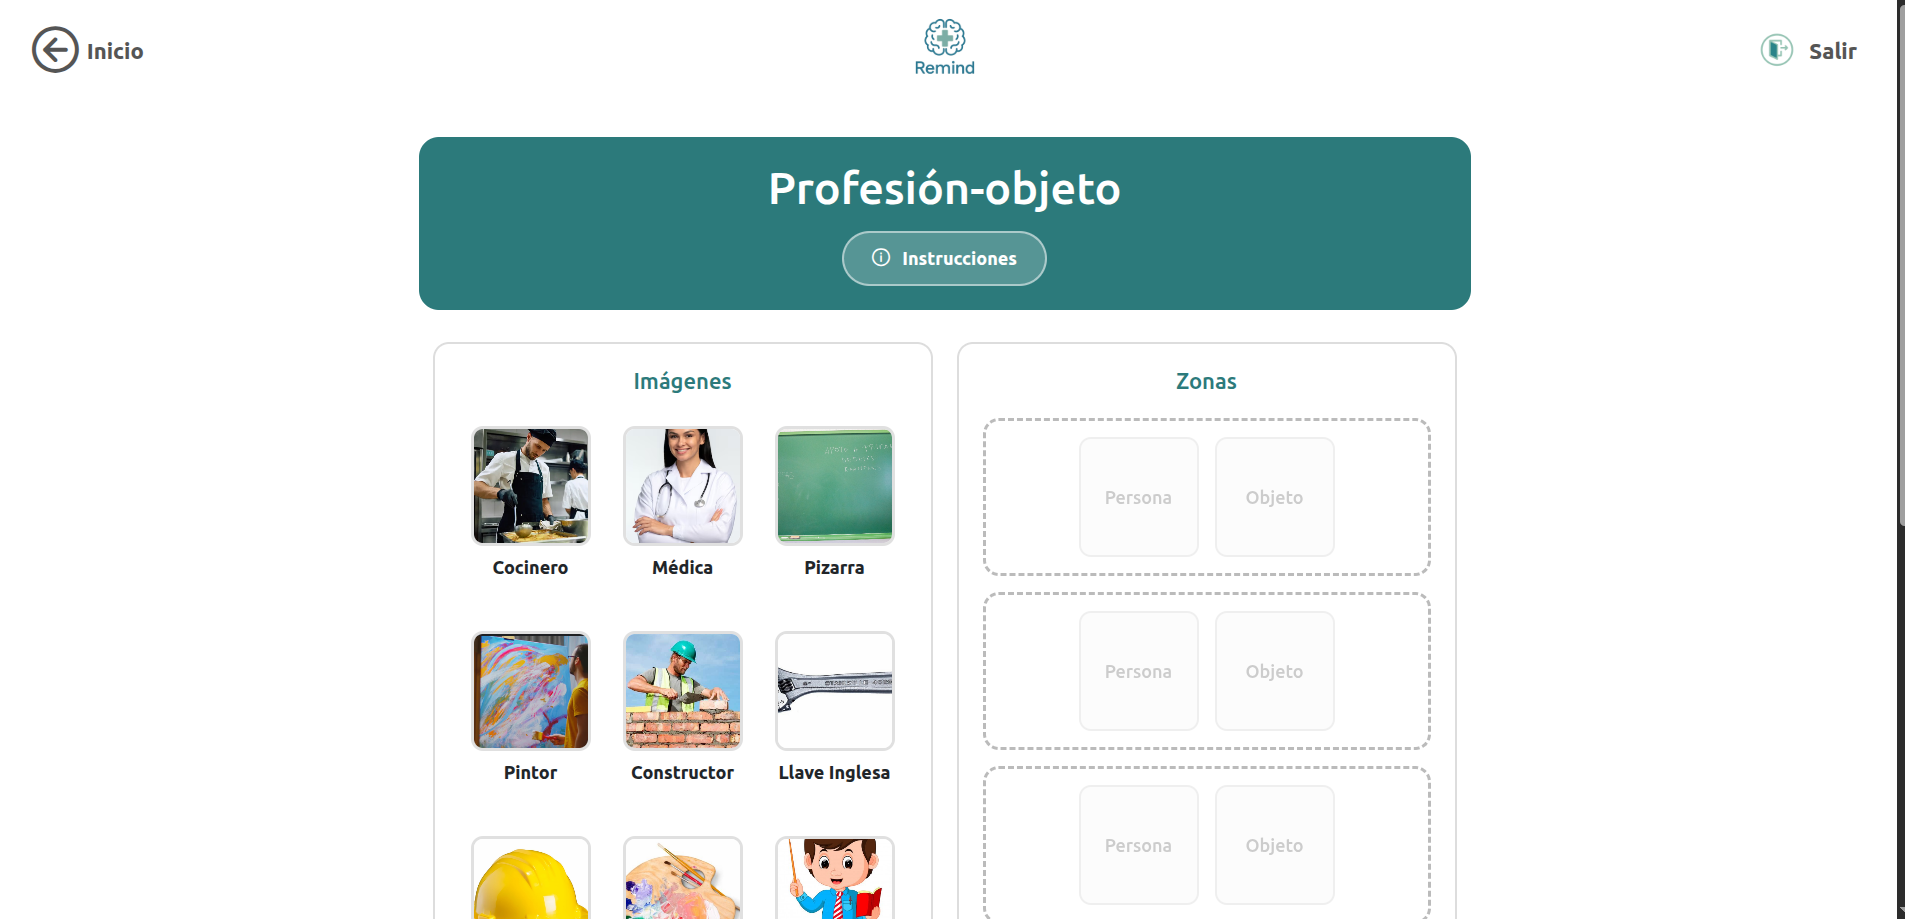
\includegraphics[width=\textwidth]{imagenes/manual/juego_unir.png}
    \caption{Juego ``Relacionar objetos y profesiones''}
\end{figure}

\subsection{Pagos exactos (El cambio)}

\begin{itemize}
    \item \textbf{Qué trabaja:} cálculo con monedas y billetes, manejo del euro.
    \item \textbf{Instrucciones en audio:} sí.
    \item \textbf{Cómo se juega:} don Manuel va a comprar pan y leche. En la pantalla aparecen monedas y billetes de distintas cantidades (1 céntimo, 2 céntimos, 5 céntimos, 10 céntimos, 20 céntimos, 50 céntimos, 1 euro, 2 euros, 5 euros, 10 euros, 20 euros y 50 euros). El paciente debe seleccionar la cantidad exacta para pagar el producto mostrado. En niveles más avanzados, debe calcular el cambio que hay que devolver.
    \item \textbf{Dificultad:} nivel fácil (pagar el importe exacto), medio (devolver cambio con cantidades pequeñas), difícil (devolver cambio con cantidades mayores).
\end{itemize}

\begin{figure}[H]
    \centering
    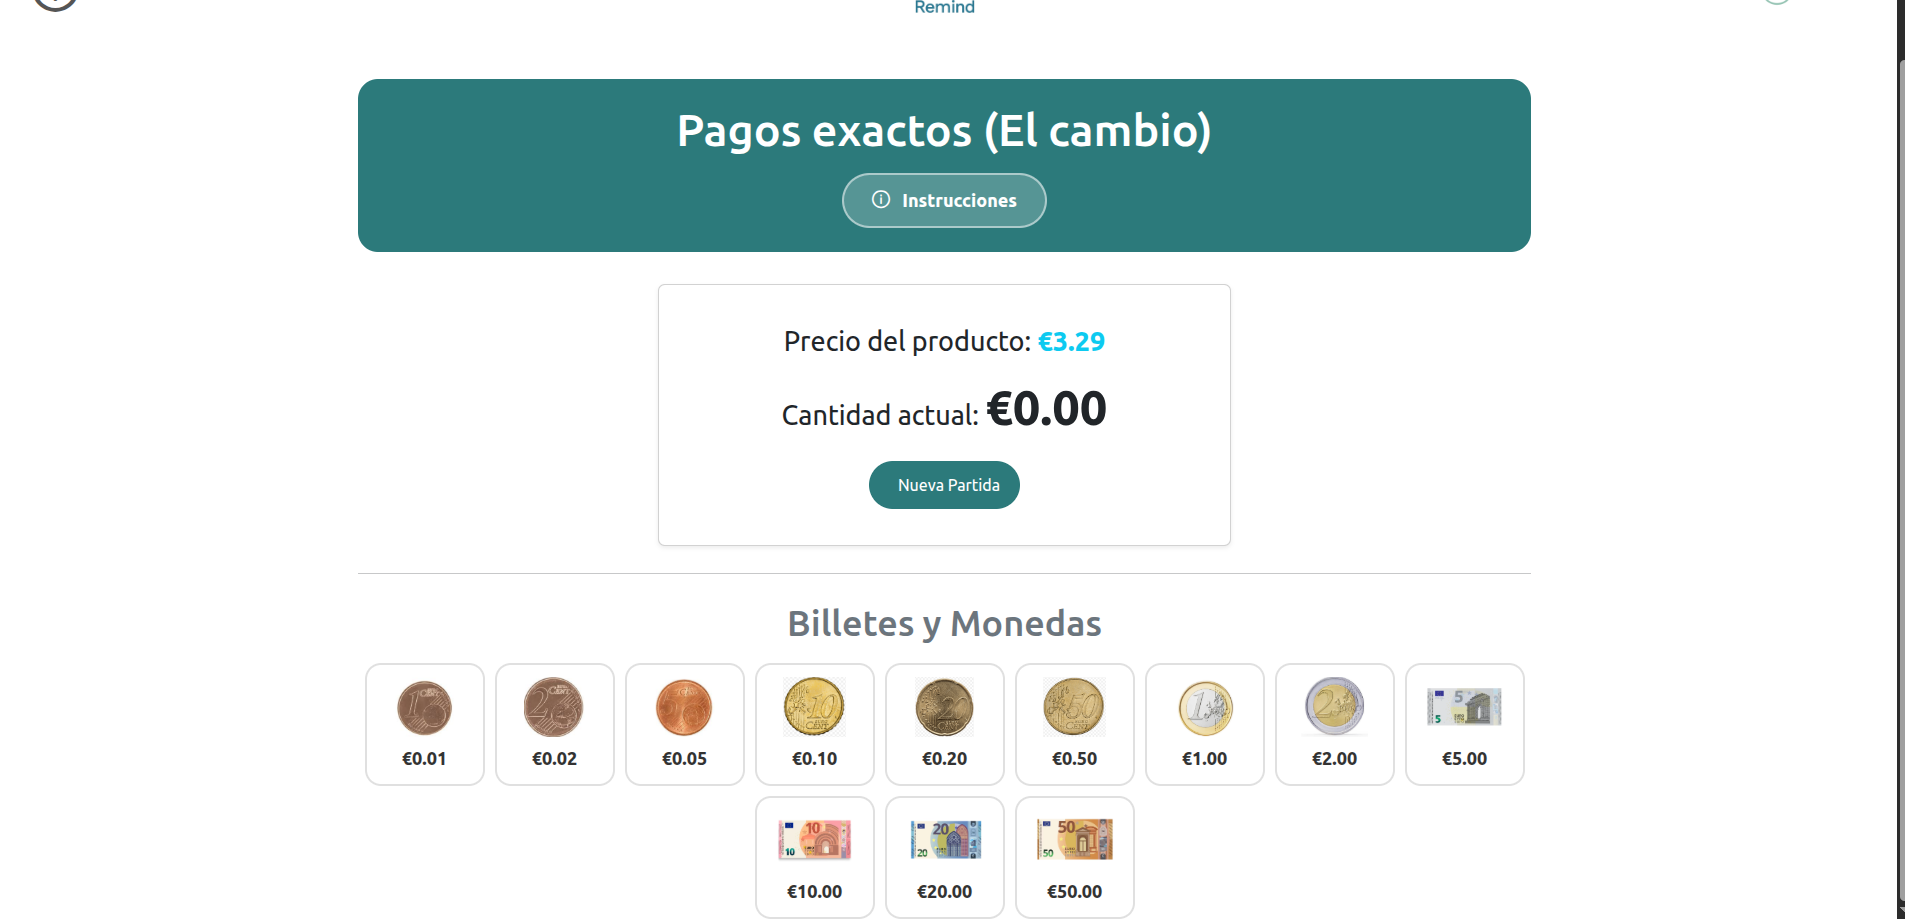
\includegraphics[width=\textwidth]{imagenes/manual/juego_cambio.png}
    \caption{Juego ``Pagos exactos (El cambio)''}
\end{figure}

\subsection{Vístete}

\begin{itemize}
    \item \textbf{Qué trabaja:} reconocimiento de prendas de vestir, orden lógico y asociación de partes del cuerpo.
    \item \textbf{Instrucciones en audio:} sí.
    \item \textbf{Cómo se juega:} hace frío y llueve. El paciente debe vestir a un personaje arrastrando cada prenda (gorro, camiseta, pantalón y zapatos) a la zona del cuerpo correspondiente, en el orden adecuado.
    \item \textbf{Dificultad:} única (4 prendas para colocar correctamente).
\end{itemize}

\begin{figure}[H]
    \centering
    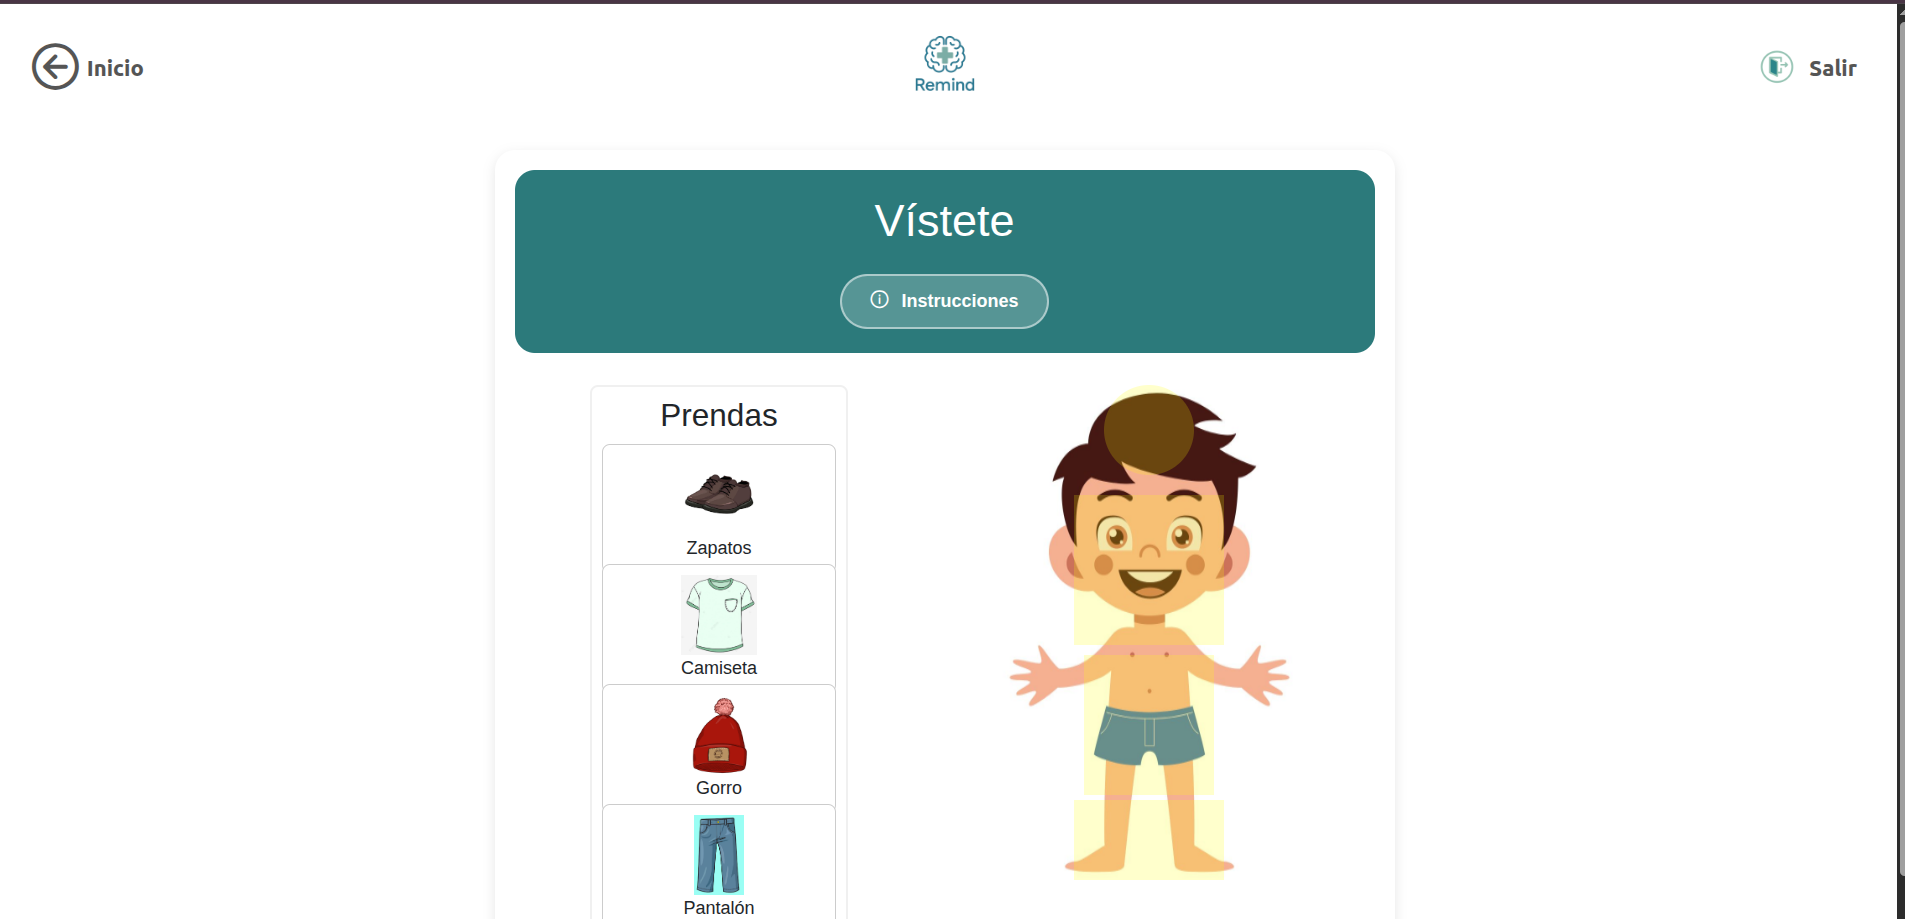
\includegraphics[width=\textwidth]{imagenes/manual/juego_vistete.png}
    \caption{Juego ``Vístete''}
\end{figure}

\subsection{Completar la oración}

\begin{itemize}
    \item \textbf{Qué trabaja:} comprensión lectora, vocabulario y gramática.
    \item \textbf{Instrucciones en audio:} sí.
    \item \textbf{Cómo se juega:} los nietos han escrito una carta pero faltan algunas palabras. El paciente debe elegir la palabra correcta entre varias opciones para completar cada frase. Al seleccionar una respuesta, el juego indica si es correcta y muestra la respuesta adecuada.
    \item \textbf{Dificultad:} nivel fácil (2 opciones), medio (3 opciones), difícil (4 opciones).
\end{itemize}

\begin{figure}[H]
    \centering
    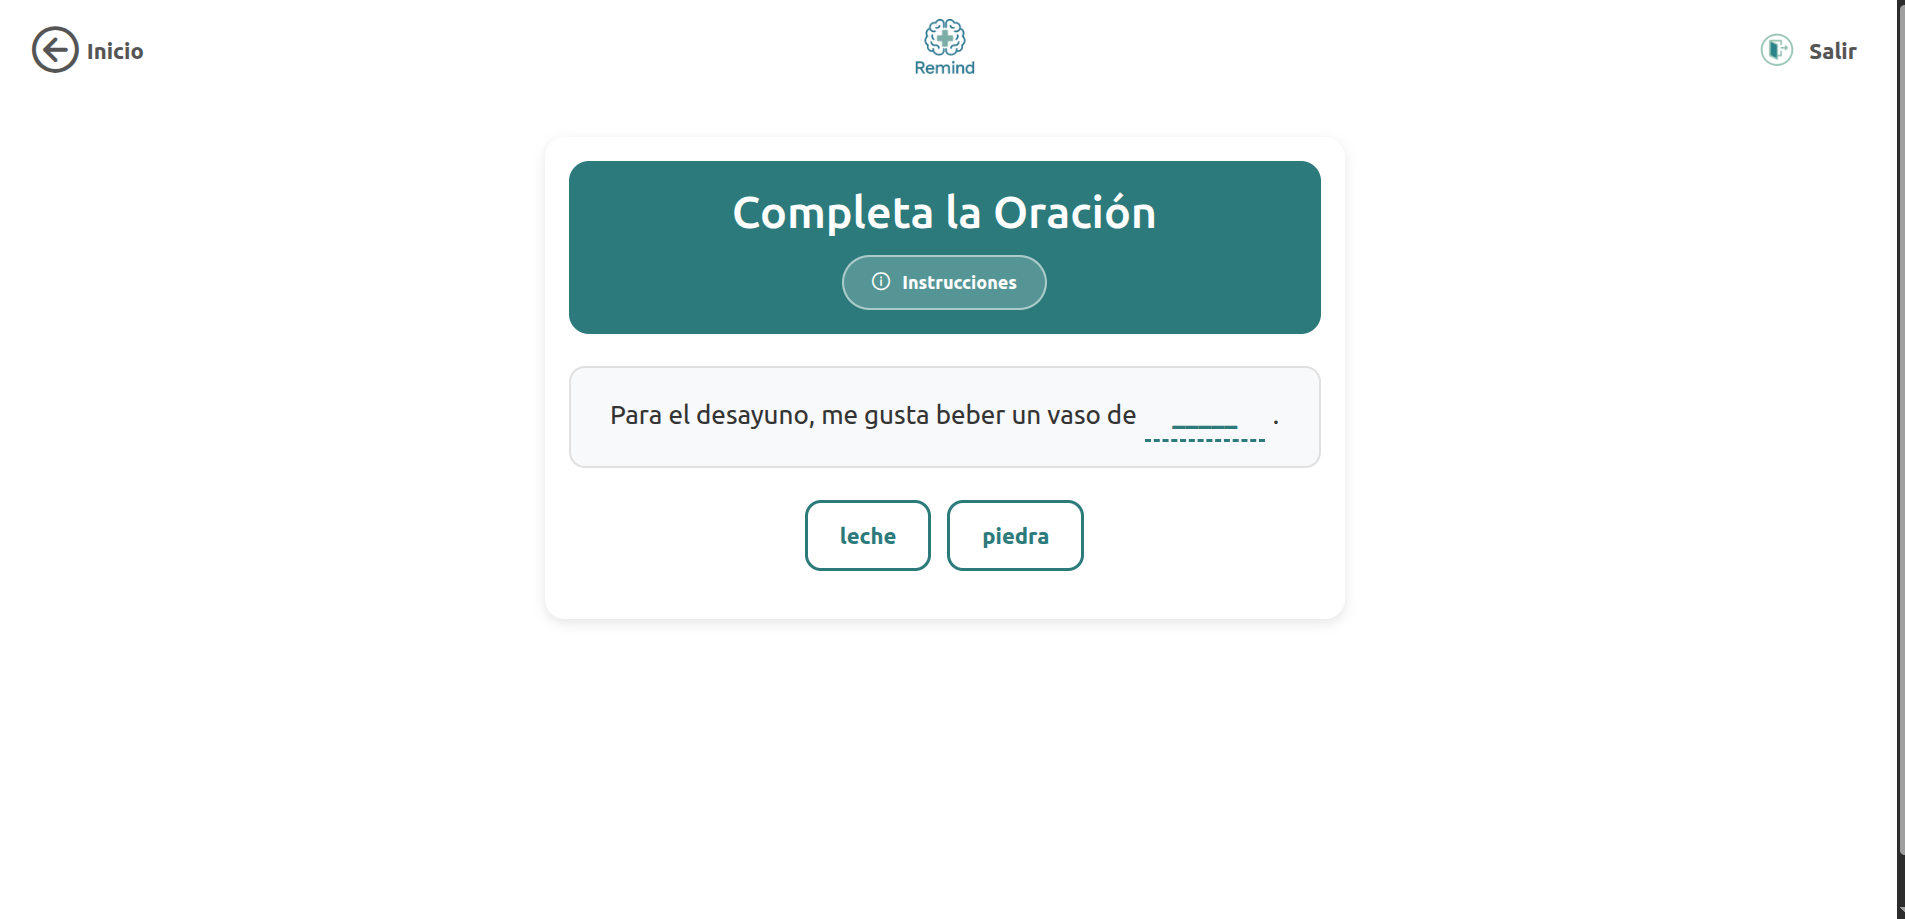
\includegraphics[width=\textwidth]{imagenes/manual/juego_oracion.png}
    \caption{Juego ``Completar la oración''}
\end{figure}

\subsection{El intruso}

\begin{itemize}
    \item \textbf{Qué trabaja:} categorización semántica, razonamiento lógico y vocabulario.
    \item \textbf{Instrucciones en audio:} sí.
    \item \textbf{Cómo se juega:} alguien ha dejado un objeto en el cajón de la cocina que no debería estar ahí. El paciente debe identificar la palabra que no pertenece al grupo (por ejemplo, entre ``manzana, pera, plátano, uva y coche'', el intruso es ``coche'' porque los demás son frutas).
    \item \textbf{Dificultad:} nivel fácil (3 palabras), medio (4 palabras), difícil (5 palabras).
\end{itemize}

\begin{figure}[H]
    \centering
    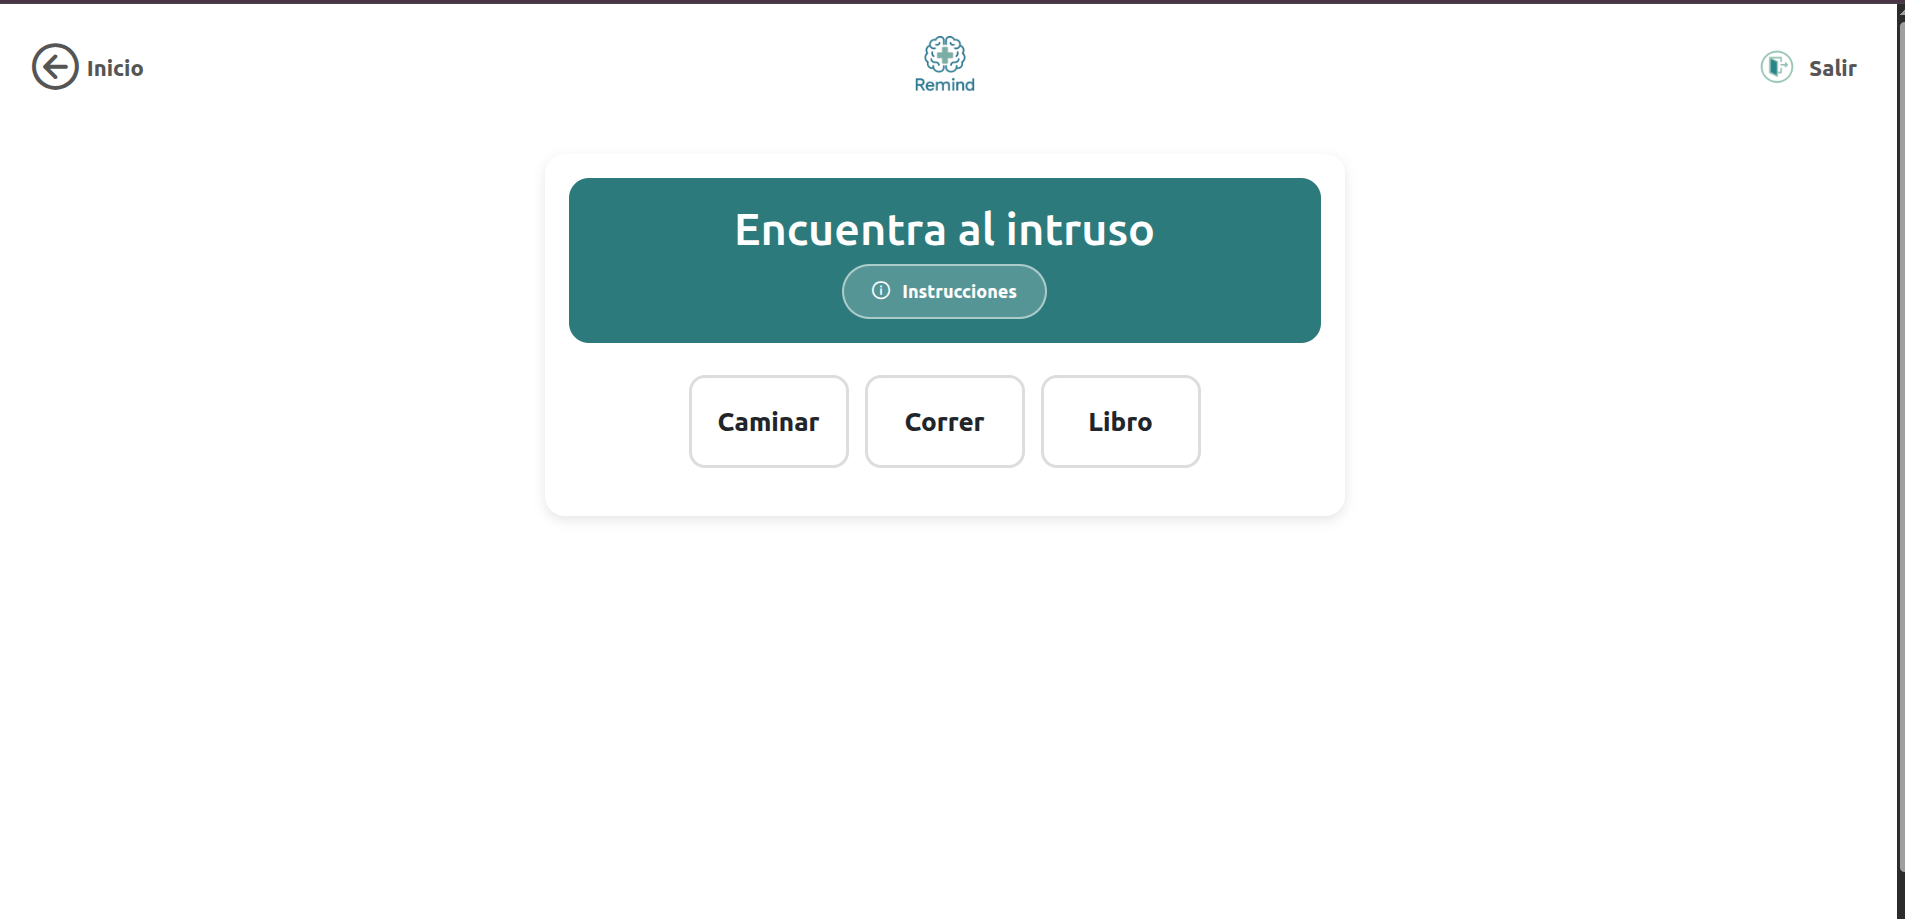
\includegraphics[width=\textwidth]{imagenes/manual/juego_instruso.png}
    \caption{Juego ``El intruso''}
\end{figure}

\subsection{Resumen de juegos}

\begin{center}
\begin{tabularx}{\textwidth}{|X|X|c|}
    \hline
    \textbf{Juego} & \textbf{Capacidad trabajada} & \textbf{Interacción} \\
    \hline
    Ordenar la secuencia & Memoria visual y ordenación & Pulsar en orden \\
    \hline
    Relacionar objetos y profesiones & Asociación semántica & Arrastrar y soltar \\
    \hline
    Pagos exactos (El cambio) & Cálculo con euros & Pulsar monedas/billetes \\
    \hline
    Vístete & Reconocimiento y orden lógico & Arrastrar y soltar \\
    \hline
    Completar la oración & Lenguaje y vocabulario & Pulsar opción \\
    \hline
    El intruso & Categorización y razonamiento & Pulsar opción \\
    \hline
\end{tabularx}
\end{center}

\subsection{Recomendaciones según el área cognitiva}

Para facilitar la labor del terapeuta a la hora de prescribir los juegos, la siguiente tabla relaciona cada capacidad cognitiva con los juegos que la trabajan:

\begin{center}
\begin{tabularx}{\textwidth}{|X|X|}
    \hline
    \textbf{Capacidad cognitiva} & \textbf{Juegos recomendados} \\
    \hline
    Memoria visual y ordenación & Ordenar la secuencia \\
    \hline
    Lenguaje y vocabulario & Completar la oración, El intruso \\
    \hline
    Cálculo y manejo del dinero & Pagos exactos (El cambio) \\
    \hline
    Razonamiento y categorización & El intruso, Relacionar objetos y profesiones \\
    \hline
    Asociación semántica & Relacionar objetos y profesiones \\
    \hline
    Praxias, orientación corporal y orden lógico & Vístete \\
    \hline
\end{tabularx}
\end{center}

\section{Solución de problemas comunes}

A continuación se indican algunas situaciones habituales y cómo resolverlas.

\subsection{Error al iniciar sesión}

Si al introducir el usuario y la contraseña aparece un mensaje de error, compruebe lo siguiente:

\begin{enumerate}
    \item Ha escrito correctamente el \textbf{nombre de usuario} (respeta mayúsculas y minúsculas).
    \item Ha escrito correctamente la \textbf{contraseña}.
    \item Si ha olvidado la contraseña, solicite al administrador o terapeuta que le genere una nueva.
\end{enumerate}

\subsection{No aparecen juegos en la agenda}

Si el paciente entra en ``Ir a mis juegos'' y ve el mensaje ``Aún no tienes juegos asignados'', significa que el terapeuta aún no le ha asignado ninguna actividad. Debe contactar con su terapeuta para que le asigne los juegos desde la sección \textbf{Agendas}.

\subsection{El juego no responde o algo falla}

Si durante una partida el juego no responde o el paciente se queda atascado:

\begin{itemize}
    \item Pulse el botón \textbf{Reiniciar} o \textbf{Nueva partida} para empezar de nuevo.
    \item Si el problema persiste, cierre la sesión y vuelva a entrar.
    \item Como último recurso, contacte con el administrador del sistema.
\end{itemize}
